%!TEX program = xelatex
% 完整编译方法 1 pdflatex -> bibtex -> pdflatex -> pdflatex
% 完整编译方法 2: xelatex -> bibtex -> xelatex -> xelatex
\documentclass[lang=cn,11pt]{elegantpaper}

\title{TCP数据段捕获与分析报告}
\author{\href{https://github.com/Jack-Lio}{李伟}}

\institute{1711350  计算机科学与技术一班}

% 不需要版本信息,直接注释即可
%\version{0.07}
% 不需要时间信息的话,需要把 \today 删除。
\date{\today}


% 如果想修改参考文献样式,请把这行注释掉
\usepackage[numbers]{gbt7714}  % 国标

\begin{document}

\maketitle

\begin{abstract}
\noindent 本实验通过WireShark捕捉实时网络数据包,并根据网络协议分析流程分析TCP的连接建立、数据传输、连接关闭的全过程,并对TCP的重要数据段进行分析,深入理解TCP的传输机制,同时在此实验中对SYN,FIN,ACK,RST,PUSH等TCP字段的作用进行了详细分析,此外在实验中对TCP keep-alive机制和快速关闭连接的机制进行了初步探索。
\keywords{TCP,WireShark,数据包捕获,数据包分析}
\end{abstract}


\section{实验要求}

通过HTTP访问某个网页,使用Wireshark对整个过程中的数据段进行捕获,分析TCP连接建立、数据传输、连接关闭的全过程,至少对其中5个典型的TCP数据段进行详细分析,给出界面截图,并同时提交捕获文件。

\section{实验环境}
\begin{itemize}
	\item 操作系统:windows10 专业版
	\item 捕获工具:WireShark 
\end{itemize}


\section{TCP数据传输机制分析}

TCP是一种面向连接的、可靠的、基于字节流的传输层通信协议,由IETF的RFC 793定义。在简化的计算机网络OSI模型中,它完成第四层传输层所指定的功能。用户数据报协议(UDP)是同一层内另一个重要的传输协议。相较于UDP,TCP的强大优势在于可靠性,TCP为上层的应用层提供了超时重传、差错检验、流量控制、拥塞控制等可靠机制,能够最大程度上保证数据端到端的可靠性。

TCP可靠性的基础很大程度上来自于TCP面向连接并维护连接状态实现的,因此了解和分析TCP建立连接以及维护连接状态的机制是十分重要的,本次实验的的主要目的就是重点分析TCP面向连接的这种机制。

TCP协议中数据的传输过程主要可以看做三个部分,分别是三次握手建立连接,数据的可靠传输,四次挥手拆除连接(部分情况下使用RESET快速拆除连接),下面主要分析这三个部分的具体细节。

\subsection{捕获数据包情况}


打开WireShark 之后点击相应的网卡设备即可针对该设备捕获数据包,默认情况下会捕获该网卡上的所有数据包,可以通过设置过滤器过滤掉非目标数据包,方便找到分析的数据包。

在本次分析中,使用的数据包保存在\text{学院网站.pcapng}文件中,数据包产生于访问学院网站的过程中,本次分析主要围绕两个TCP连接进行,第一条TCP连接的过滤器设置为\text{ip.addr == 222.30.45.190 \&\&tcp.port==443},第二条TCP连接的过滤器为\text{ip.addr == 54.223.158.33 \&\& tcp.port==80},通过筛选之后可以分别看到\figref{fig:1},\figref{fig:2}所示的数据包捕获界面。


\begin{figure}[htbp]
	\centering
	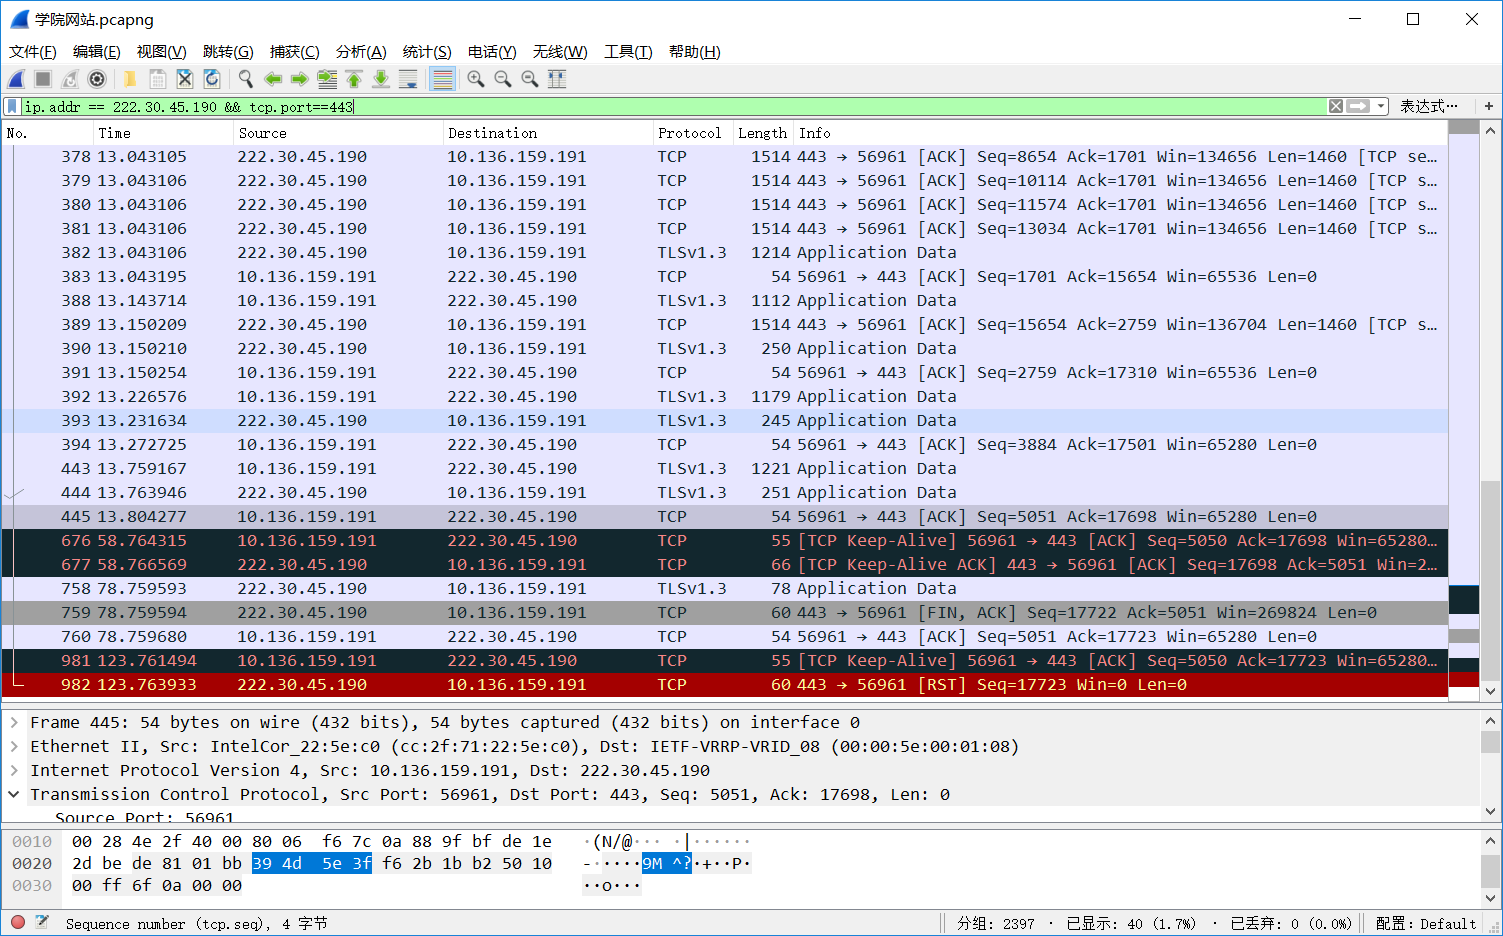
\includegraphics[width=0.6\textwidth]{con1}
	\caption{TCP连接1 \label{fig:1}}
\end{figure}
\begin{figure}[htbp]
	\centering
	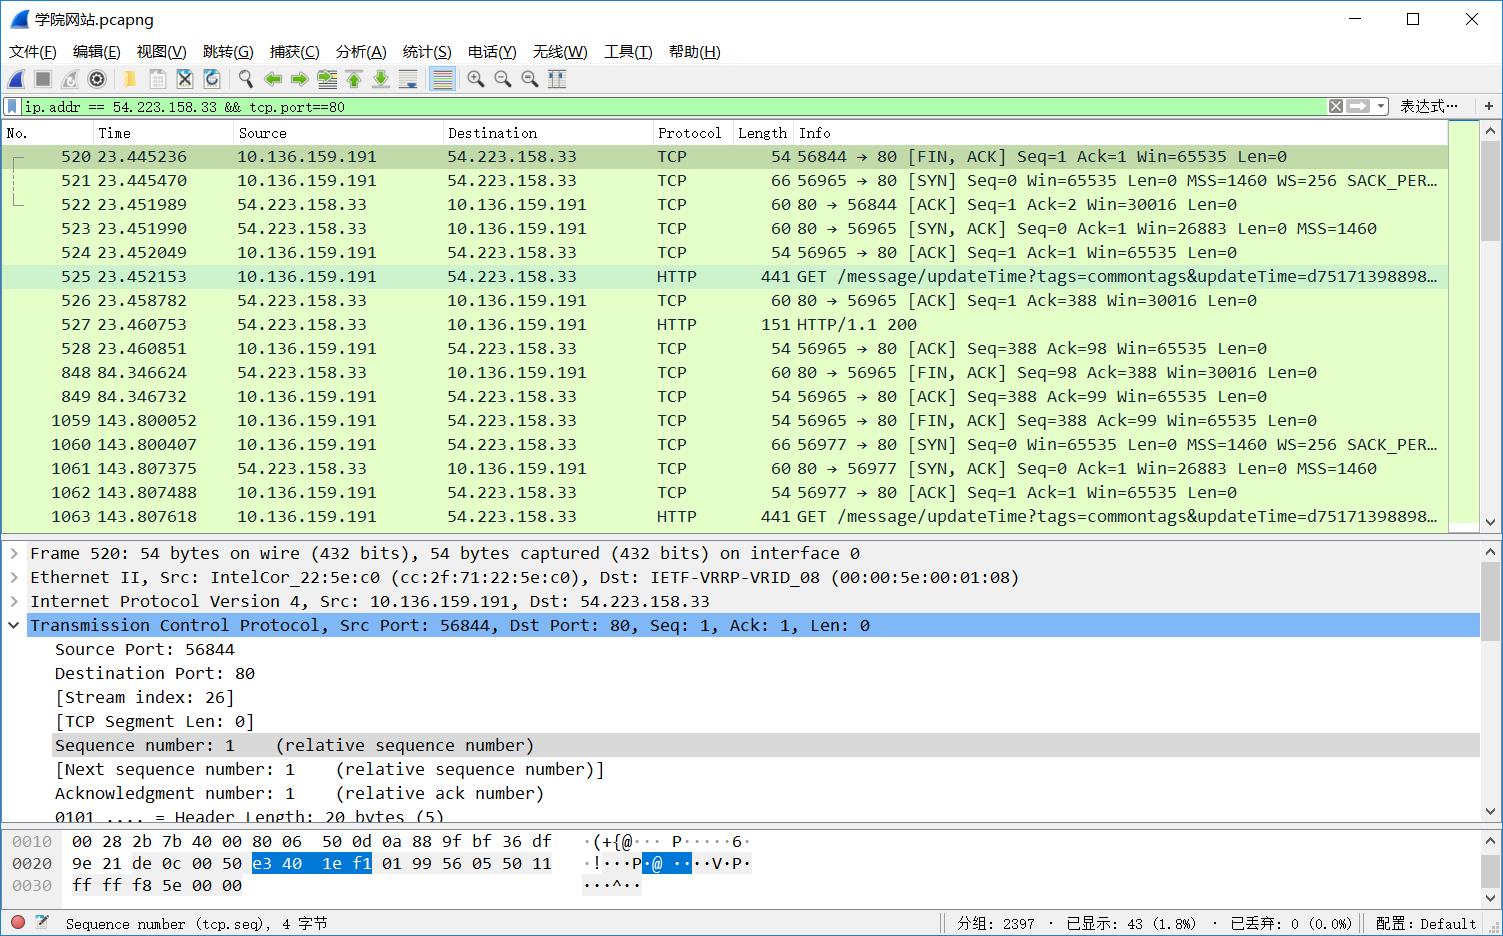
\includegraphics[width=0.8\textwidth]{con2}
	\caption{TCP连接2 \label{fig:2}}
\end{figure}


其中由于TCP连接1中出现的关于TCP相关的特殊情况较多,所以在下面的分析主要以TCP连接1作为分析对象,但由于TCP连接1中的连接拆除部分使用的是RESET直接拆除,而不是普遍的四次挥手形式,所以在链接拆除部分四次挥手将以TCP连接2作为分析对象。

\subsection{三次握手建立连接}
三次握手的详细分析基于TCP连接1的数据包进行,三次握手的过程简单描述一下就是客户端首先发起一个连接请求,其中标志位置位SYN位,服务器端接收到连接请求之后会回送一个ACK|SYN报文确认接收到连接请求并同意建立连接,之后客户端回送一个ACK确认报文,确认连接建立并通知服务器端链路连接正常。三次握手的数据包捕获截图如\figref{fig:3}所示:


\begin{figure}[htbp]
	\centering
	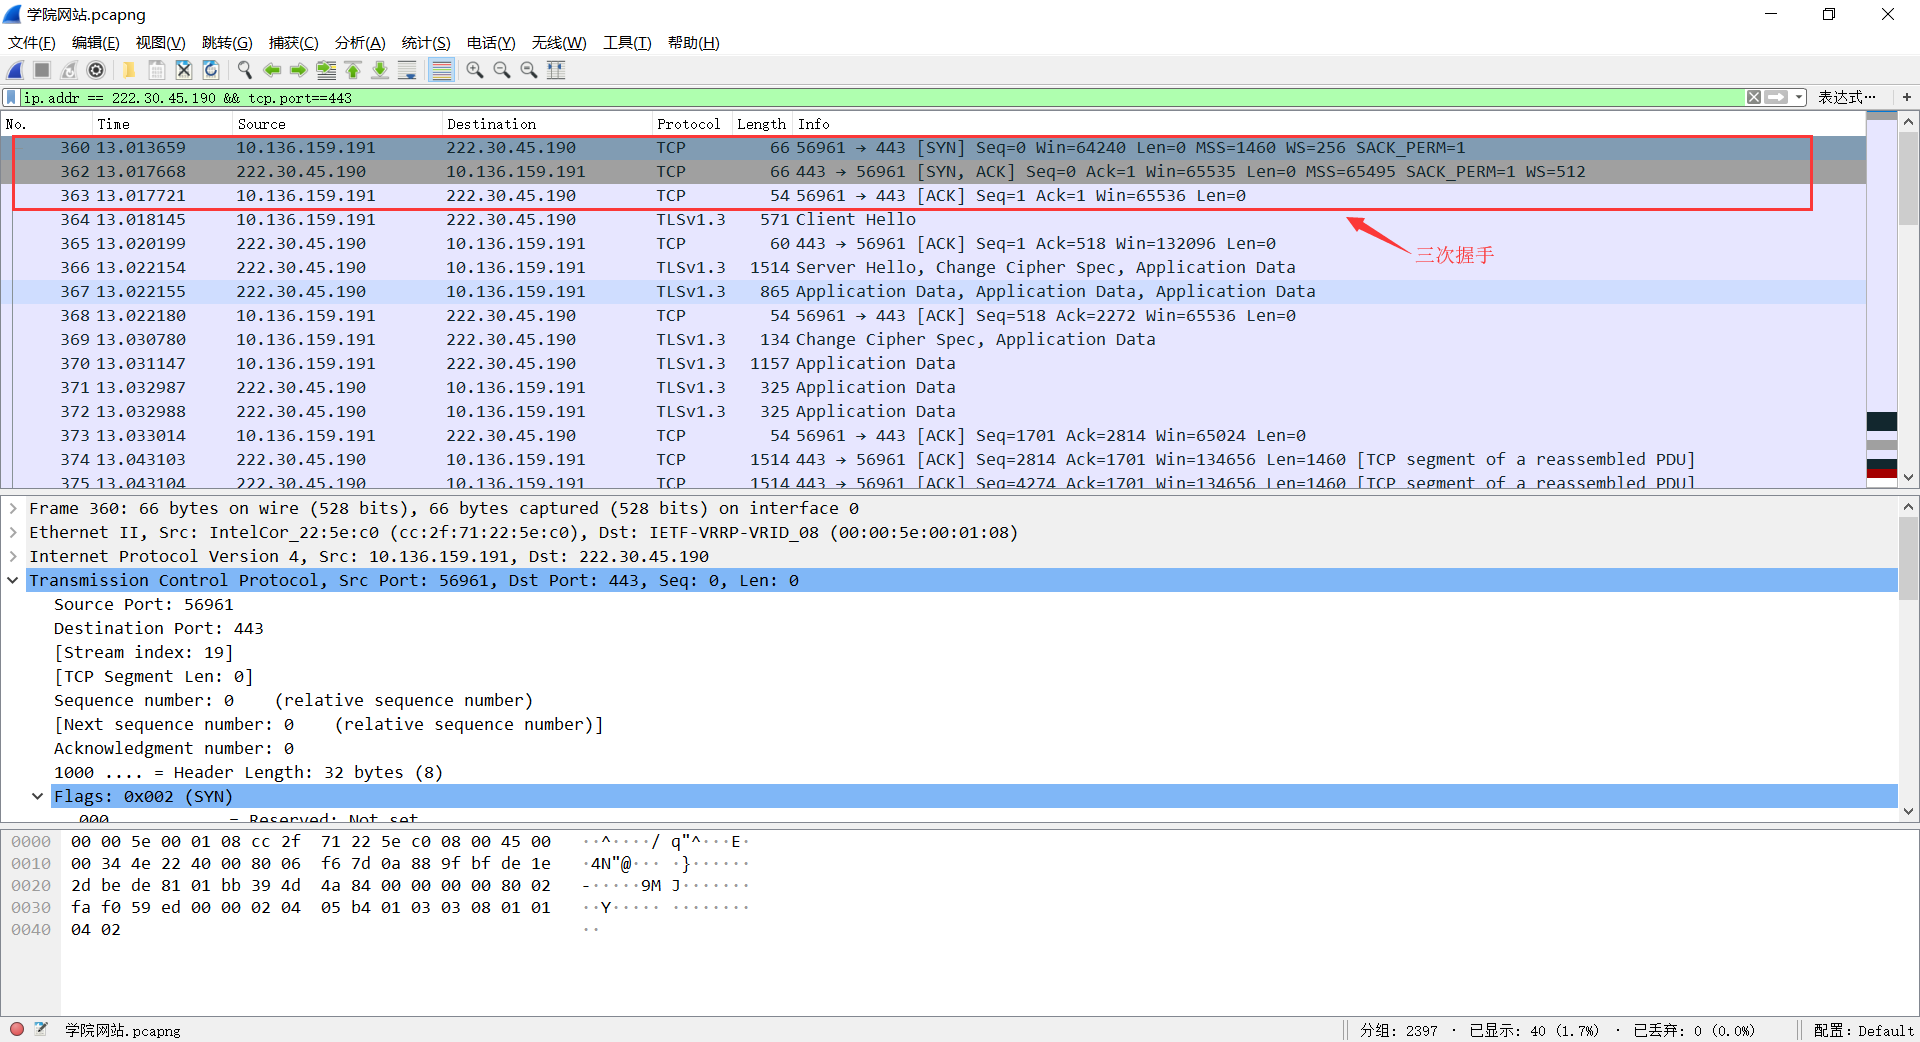
\includegraphics[width=0.8\textwidth]{三次握手}
	\caption{三次握手建立连接数据包\label{fig:3}}
\end{figure}


之所以要经过三次握手才建立连接,目的在于充分保证TCP连接的可靠性,为了防止已经失效的连接请求报文突然又传送到了服务器,导致产生错误,因此单次握手建立连接不可靠,第一次握手确认了从A到B的发送可靠性,第二次握手确定了从B到A的发送可靠性以及B的接收可靠性,第三次握手确定了A的接收可靠性并在此确定了TCP连接的稳定性,所以通过三次连接能够很好地检验TCP连接的稳定性和可靠性。TCP建立连接的三次握手示意图如\figref{fig:4}。
\begin{figure}[htbp]
	\centering
	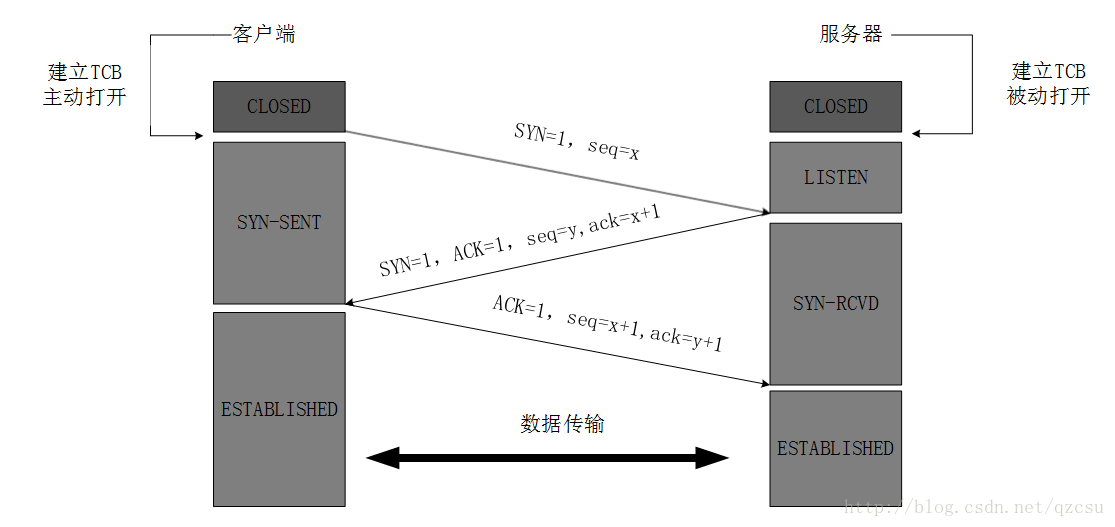
\includegraphics[width=0.6\textwidth]{三次握手示意图}
	\caption{三次握手建立连接示意图\label{fig:4}}
\end{figure}
\subsubsection{第一次握手}
第一次握手是客户端发送一条SYN标志的报文给服务端,数据包的具体信息如\figref{fig:5}所示:


\begin{figure}[htbp]
		\centering
		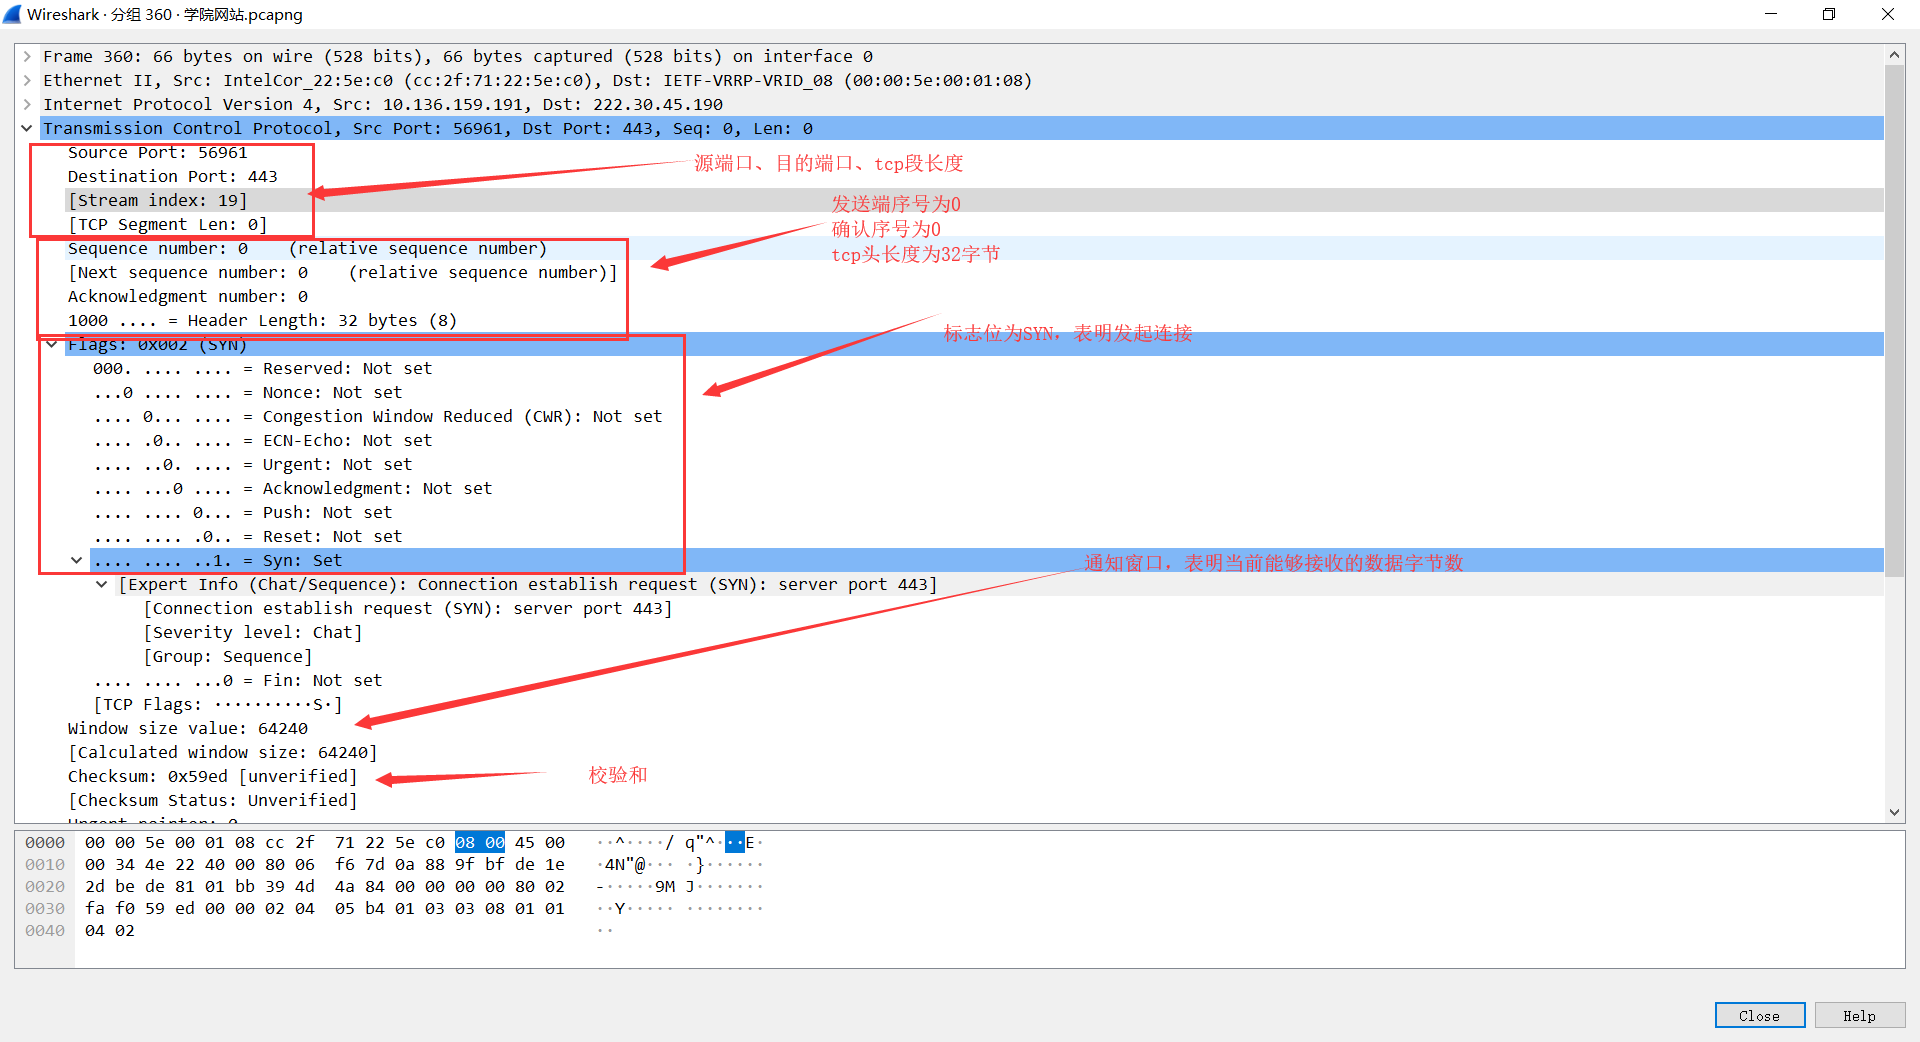
\includegraphics[width=0.8\textwidth]{SYN1}
		\centering
		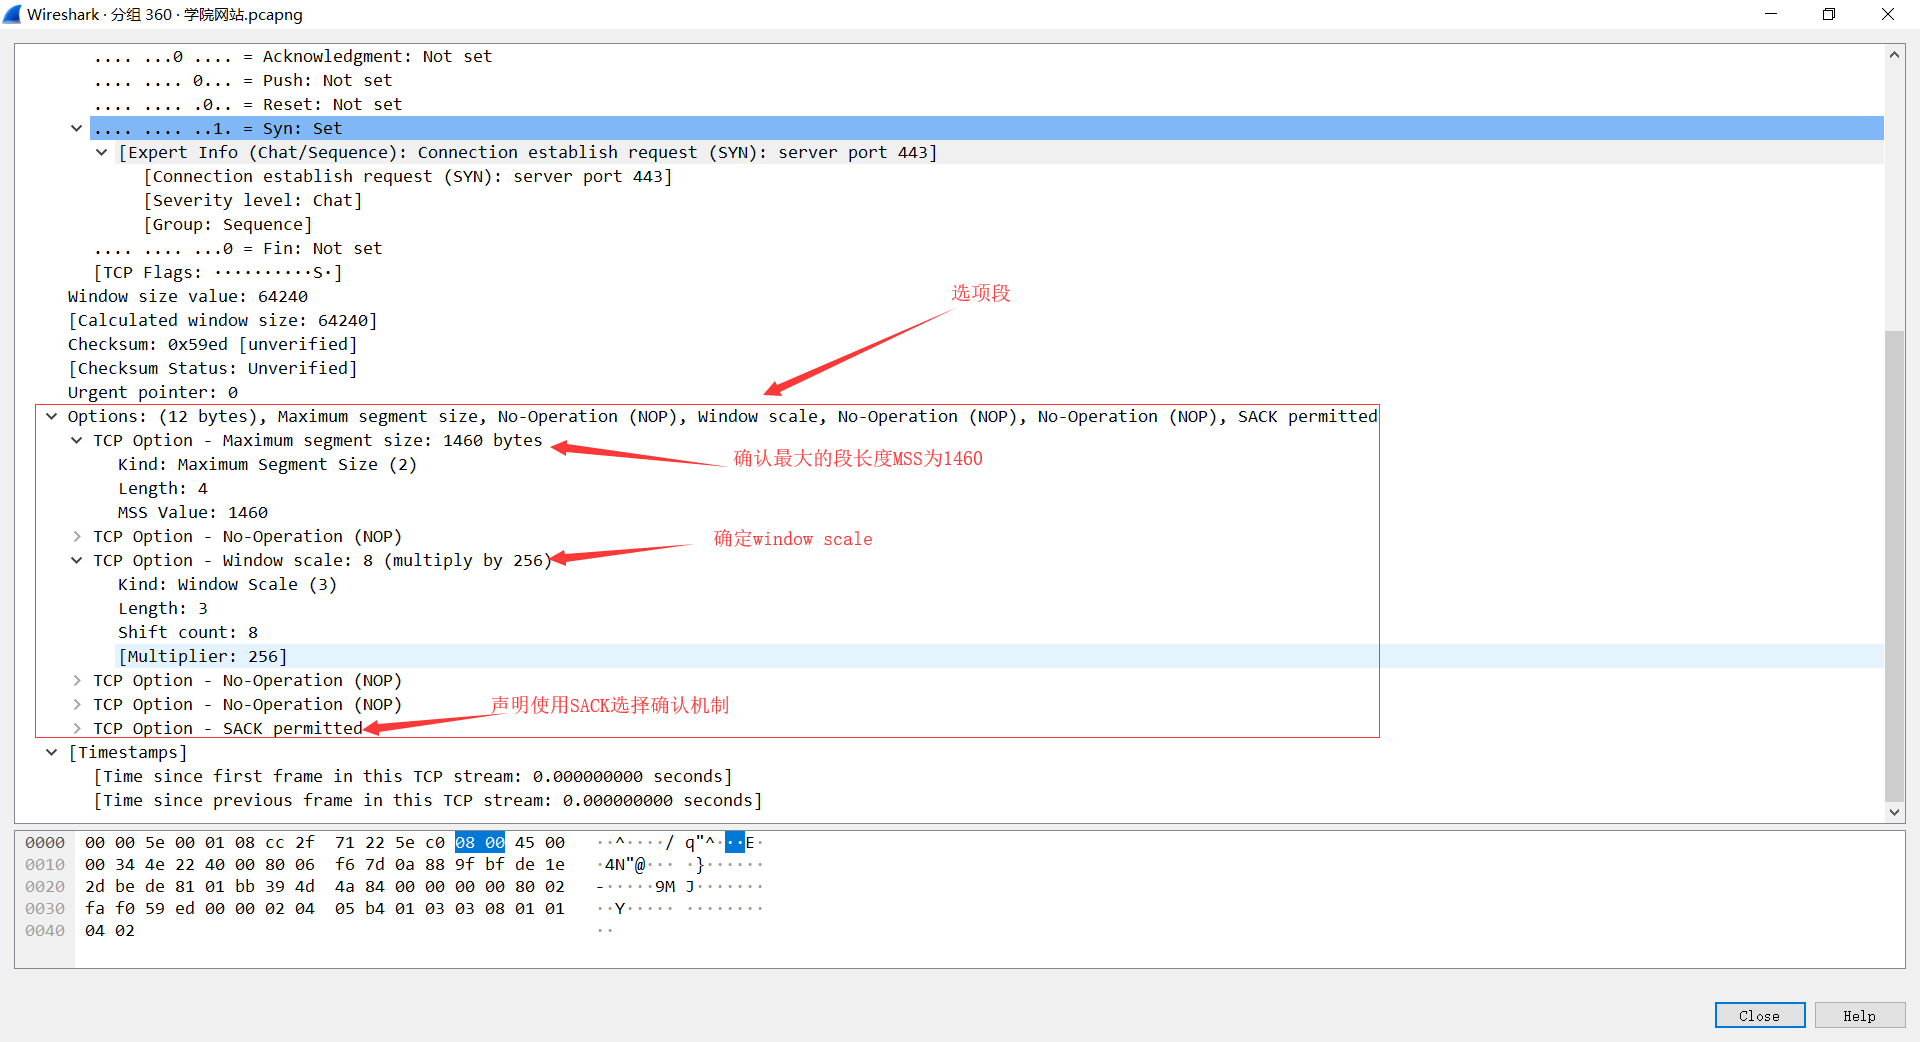
\includegraphics[width=0.8\textwidth]{SYN1-op}
		\caption{第一次握手数据包分析截图 \label{fig:5}}
\end{figure}


在第一次握手过程中,客户端会首先发送一条不带数据体的TCP报文,并选择自己的发送序列号,在这里,选取了默认的0,同时会将flags 标志位中的SYN位置位为1,说明发起连接的请求,同时在TCP头部中我们还可以看到整个TCP头部的长度为32个字节,一般来说TCP头部为20个字节,超过20字节说明包含选项。在\figref{fig:5}中我们还可以看到校验和位,以及选项options的设置,在这条连接请求中,包含了一个MSS的确定(MSS=1460),同时还设置了窗口的规模,即window scale设置,以及确定使用SACK选择确认的机制。

初次之外,可以看到在WireShark中能够看到时间戳的记录,这部分的作用在后面会说到。
\subsubsection{第二次握手}
第二次握手是服务器接收到客户端的连接请求后发送一条SYN|SCK置位的空数据报文给客户端,如\figref{fig:6}所示:

\begin{figure}[htbp]
	\centering
	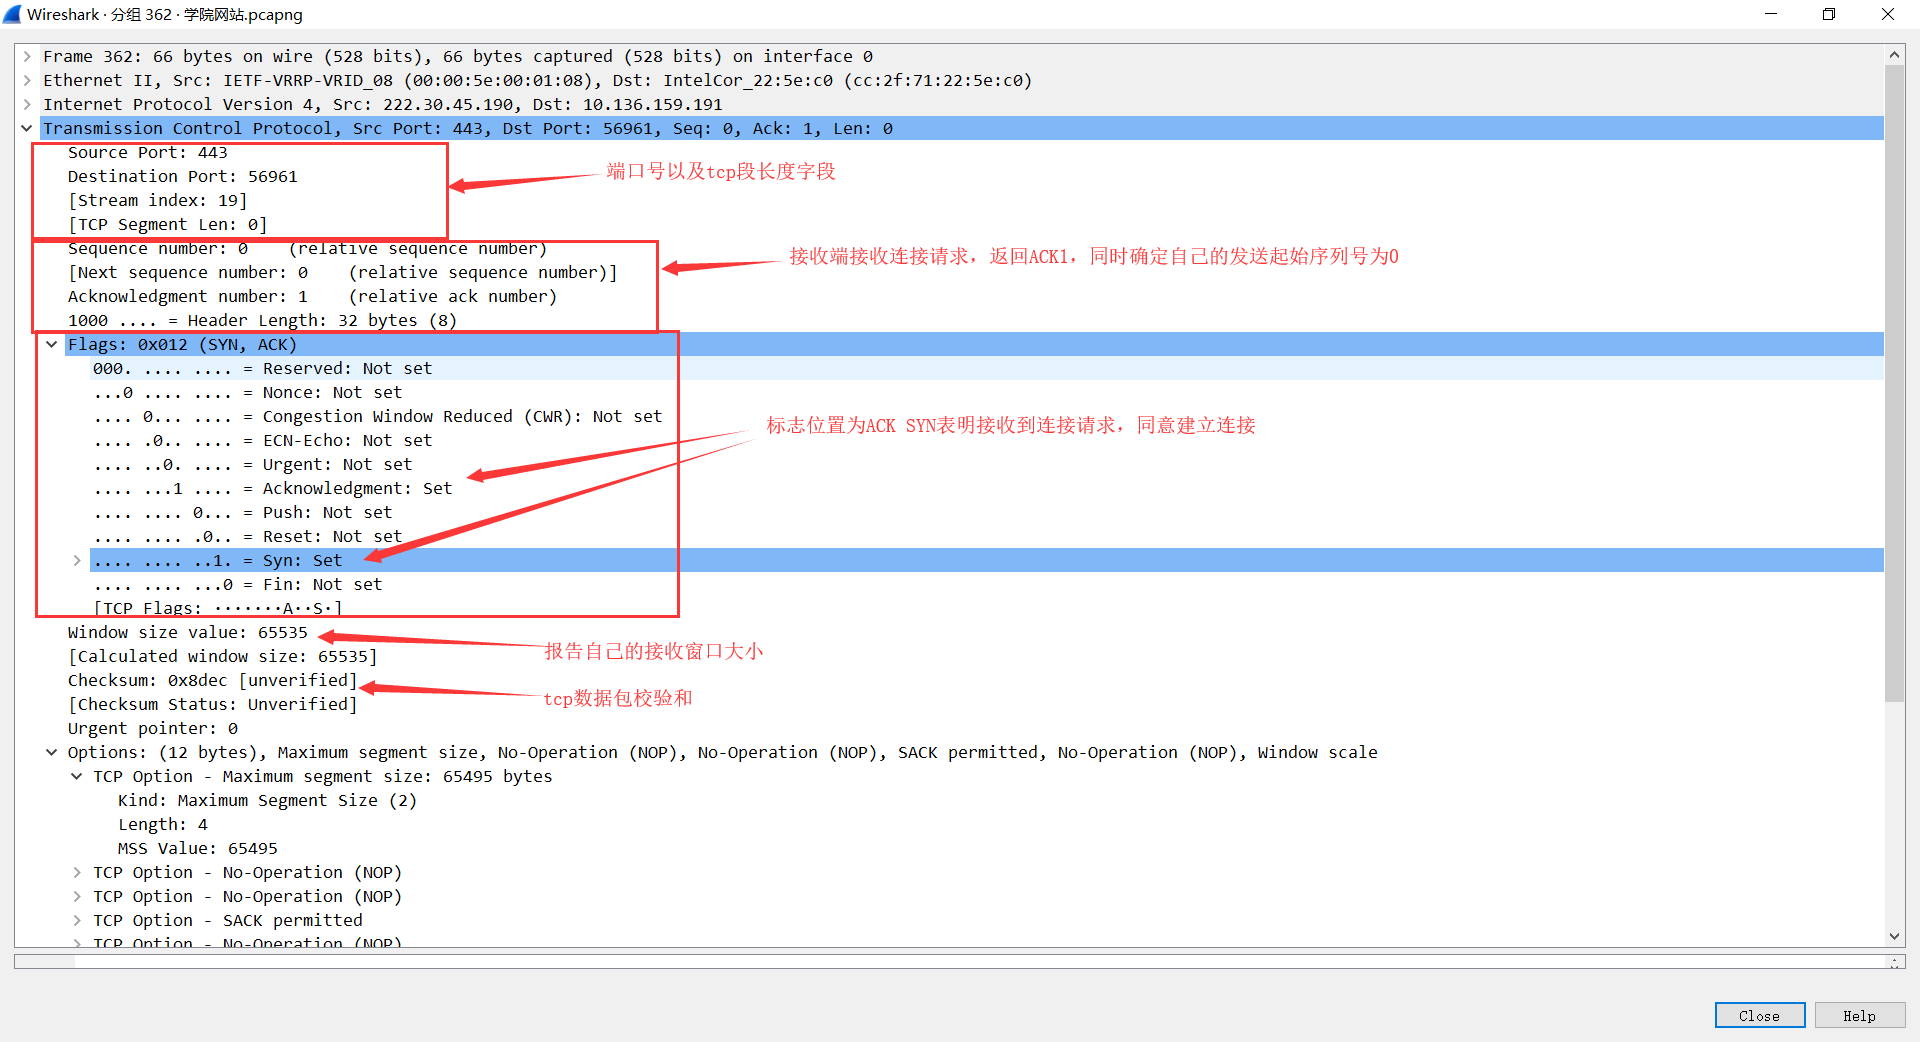
\includegraphics[width=0.8\textwidth]{SYNACK1}
	\centering
	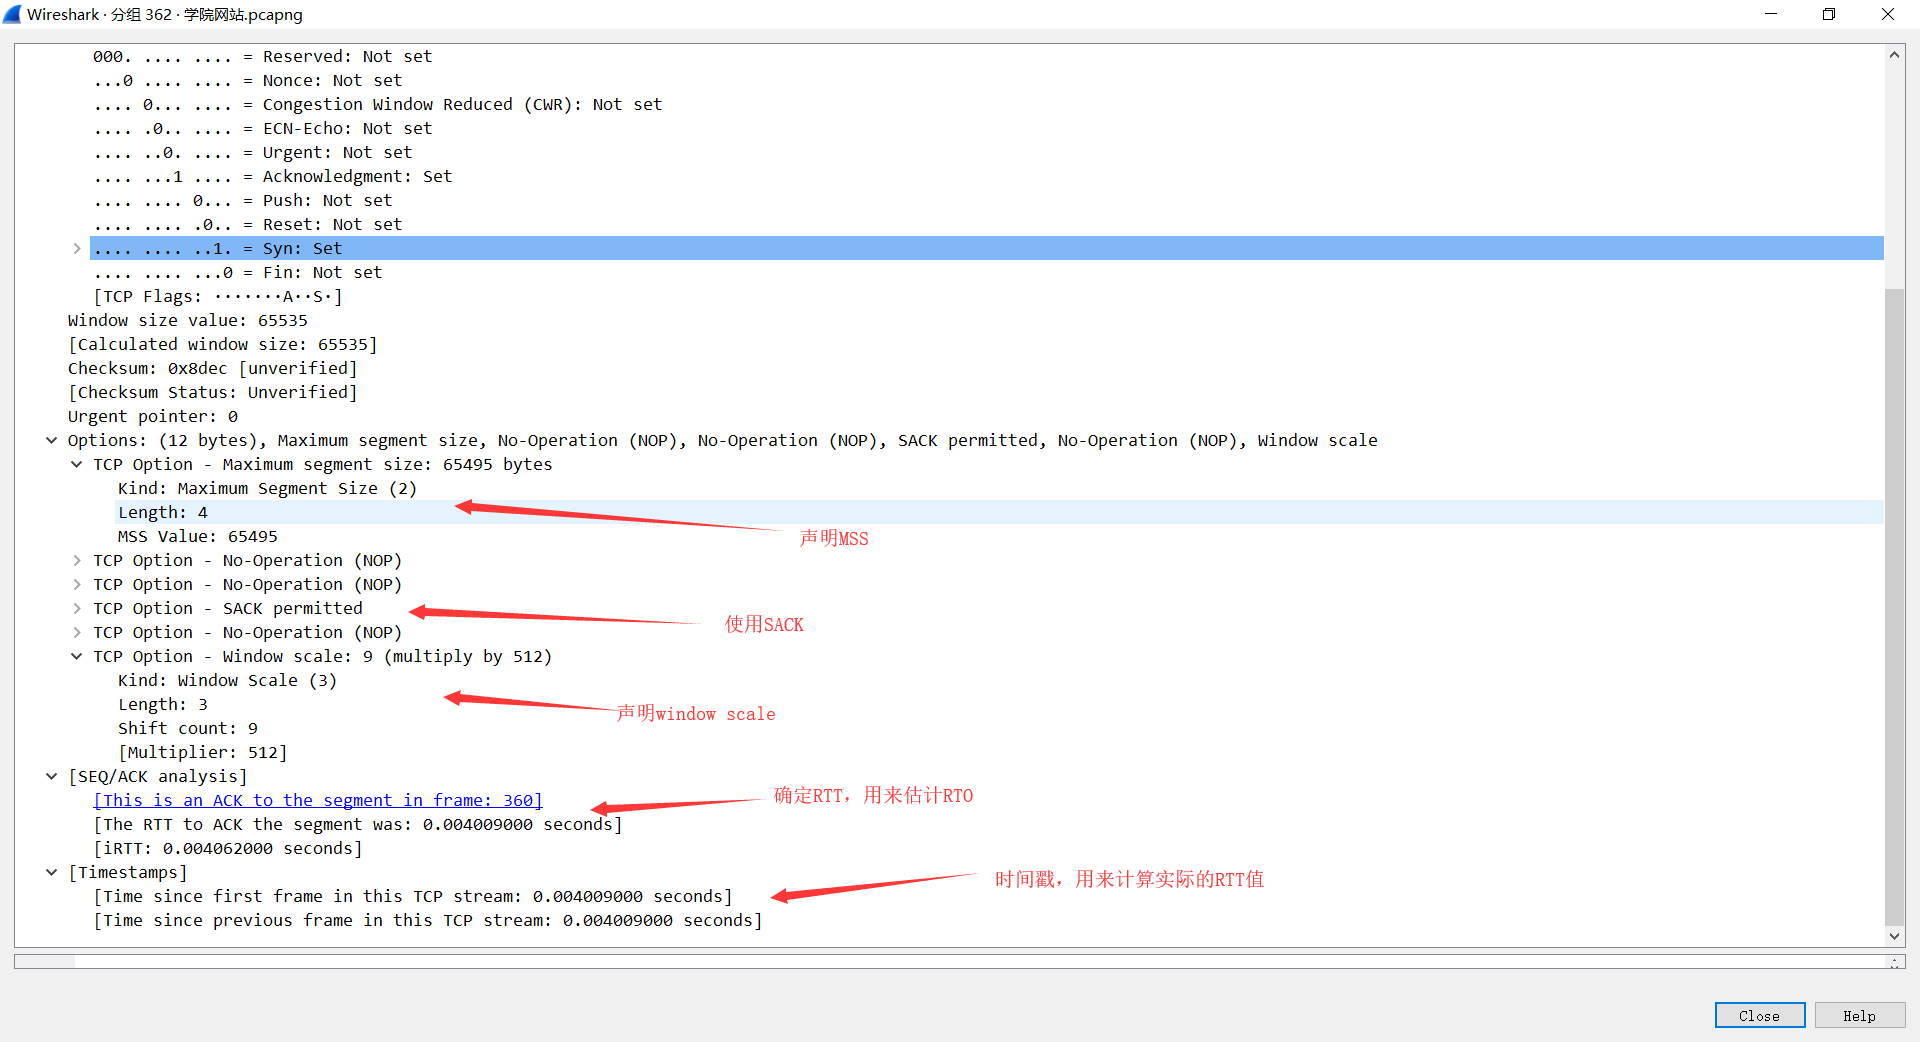
\includegraphics[width=0.8\textwidth]{SYNACKop}
	\caption{第二次握手数据包分析截图 \label{fig:6}}
\end{figure}

从截图中不难看出第二次握手中,服务器端也确定了自己的发送基础序号,这里仍然使用的是默认的0,同时确认序号为1(即第一次握手报文的发送序号加1),同时也能够看到Flags中SYN与SCK为均置为1,表明是对连接请求的回复,说明了服务器端同意建立连接。同样的,在条报文中,服务器也报告了自己的接收窗口大小,以及在选项中确定了自己的window scale,MSS,明确了使用SACK的选择确认机制。


注意到,在最后,由于发送和接收数据包,所以客户端就能够通过这两次握手确定RTT的实际大小,从而估算RTO,用来实现超时重传机制。

\subsubsection{第三次握手}
第三次的握手为客户端发送一条ACK给服务器,说明自己接收到了服务器的回复,数据包的解析如\figref{fig:7}:

\begin{figure}[htbp]
	\centering
	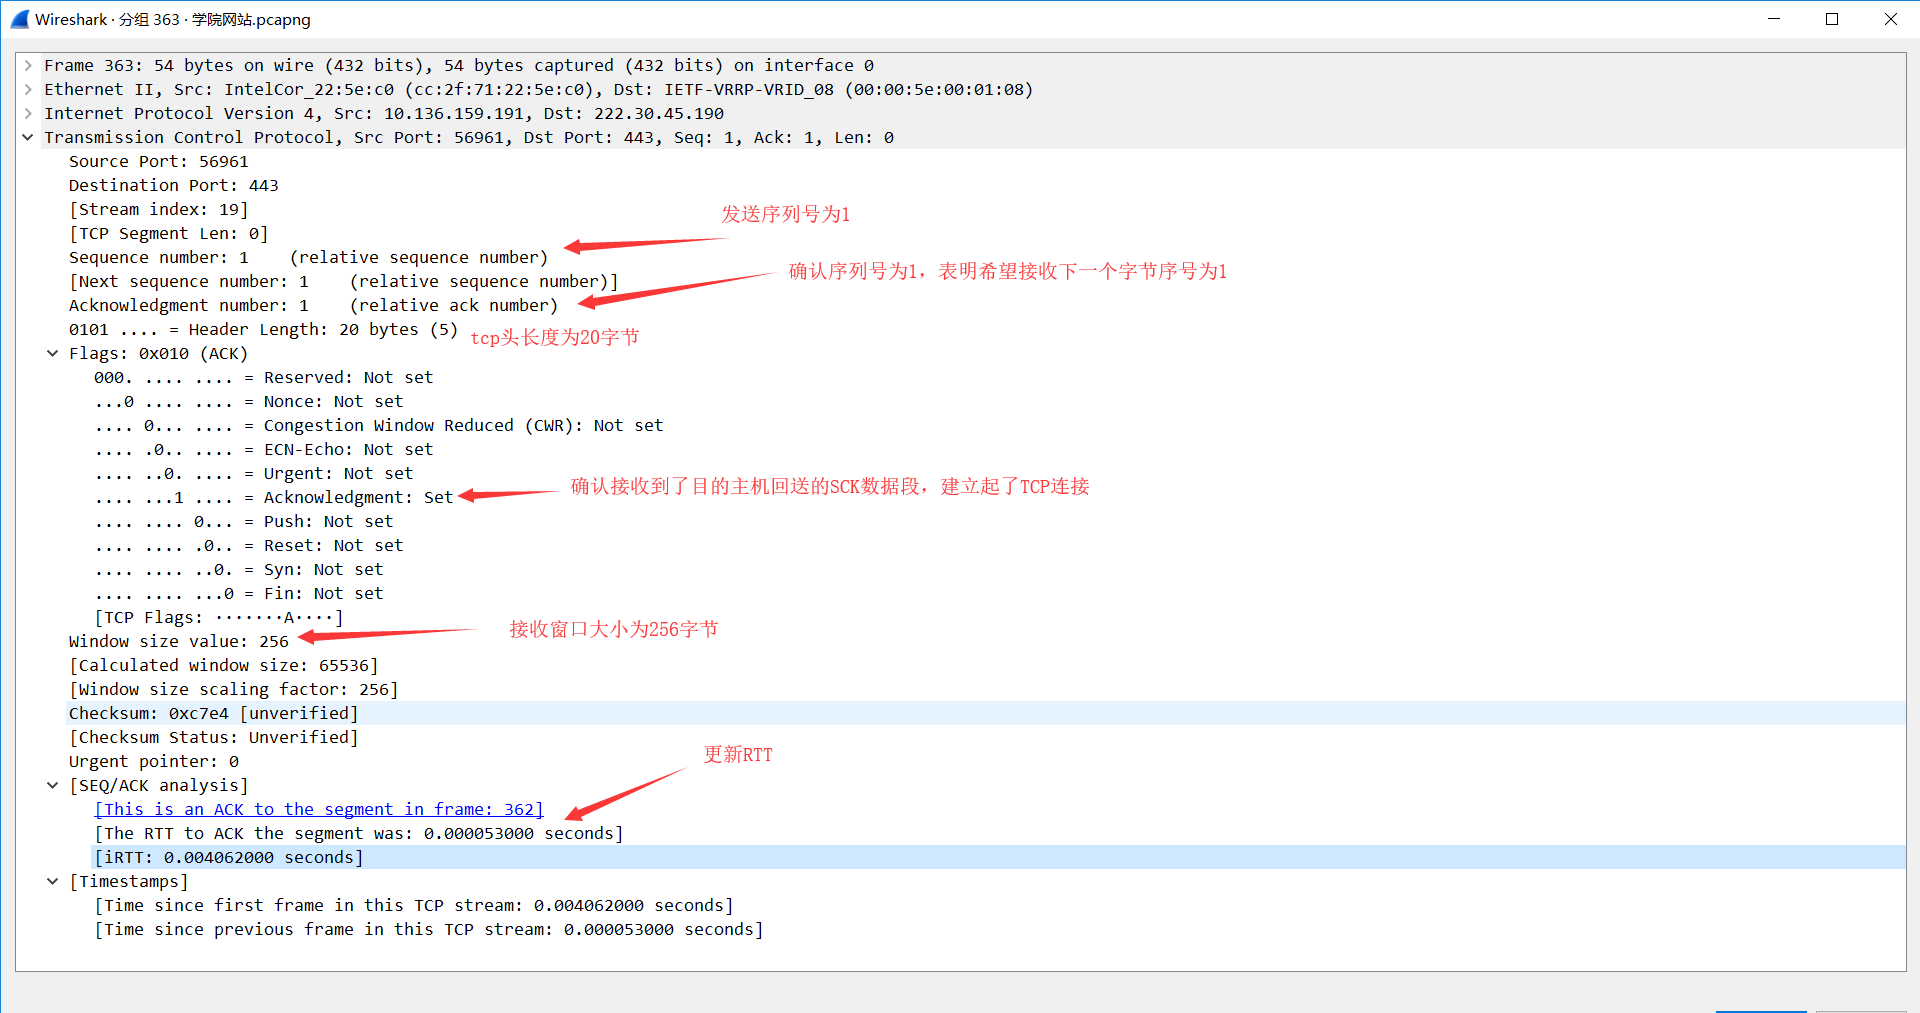
\includegraphics[width=0.6\textwidth]{ACK2}
	\caption{第三次握手数据包分析截图 \label{fig:7}}
\end{figure}

从报文中可以看到,回复的确认序列号为服务器发送序列号+1,同时自己的发送序列号为第一次发送序列号+1,Flags中ACK置位为1,说明为ACK回复报文。

特别的,在最后可以看到经过后两次握手之后,服务器端也获得了一个完整的收发过程,能够得到第一次收发的RTT数据,并估计下一次的RTT和RTO,实现超时重传的机制。

\subsection{数据传输过程}

TCP连接建立之后,客户端和服务器端通过彼此的收发数据包进行数据交互,严格按照序列号的顺序以及窗口大小的约束进行数据的发送与接收,在这里主要说明两种情况下的数据收发,用来体现型的TCP数据流情况,如\figref{fig:10}。

\begin{figure}[htbp]
	\centering
	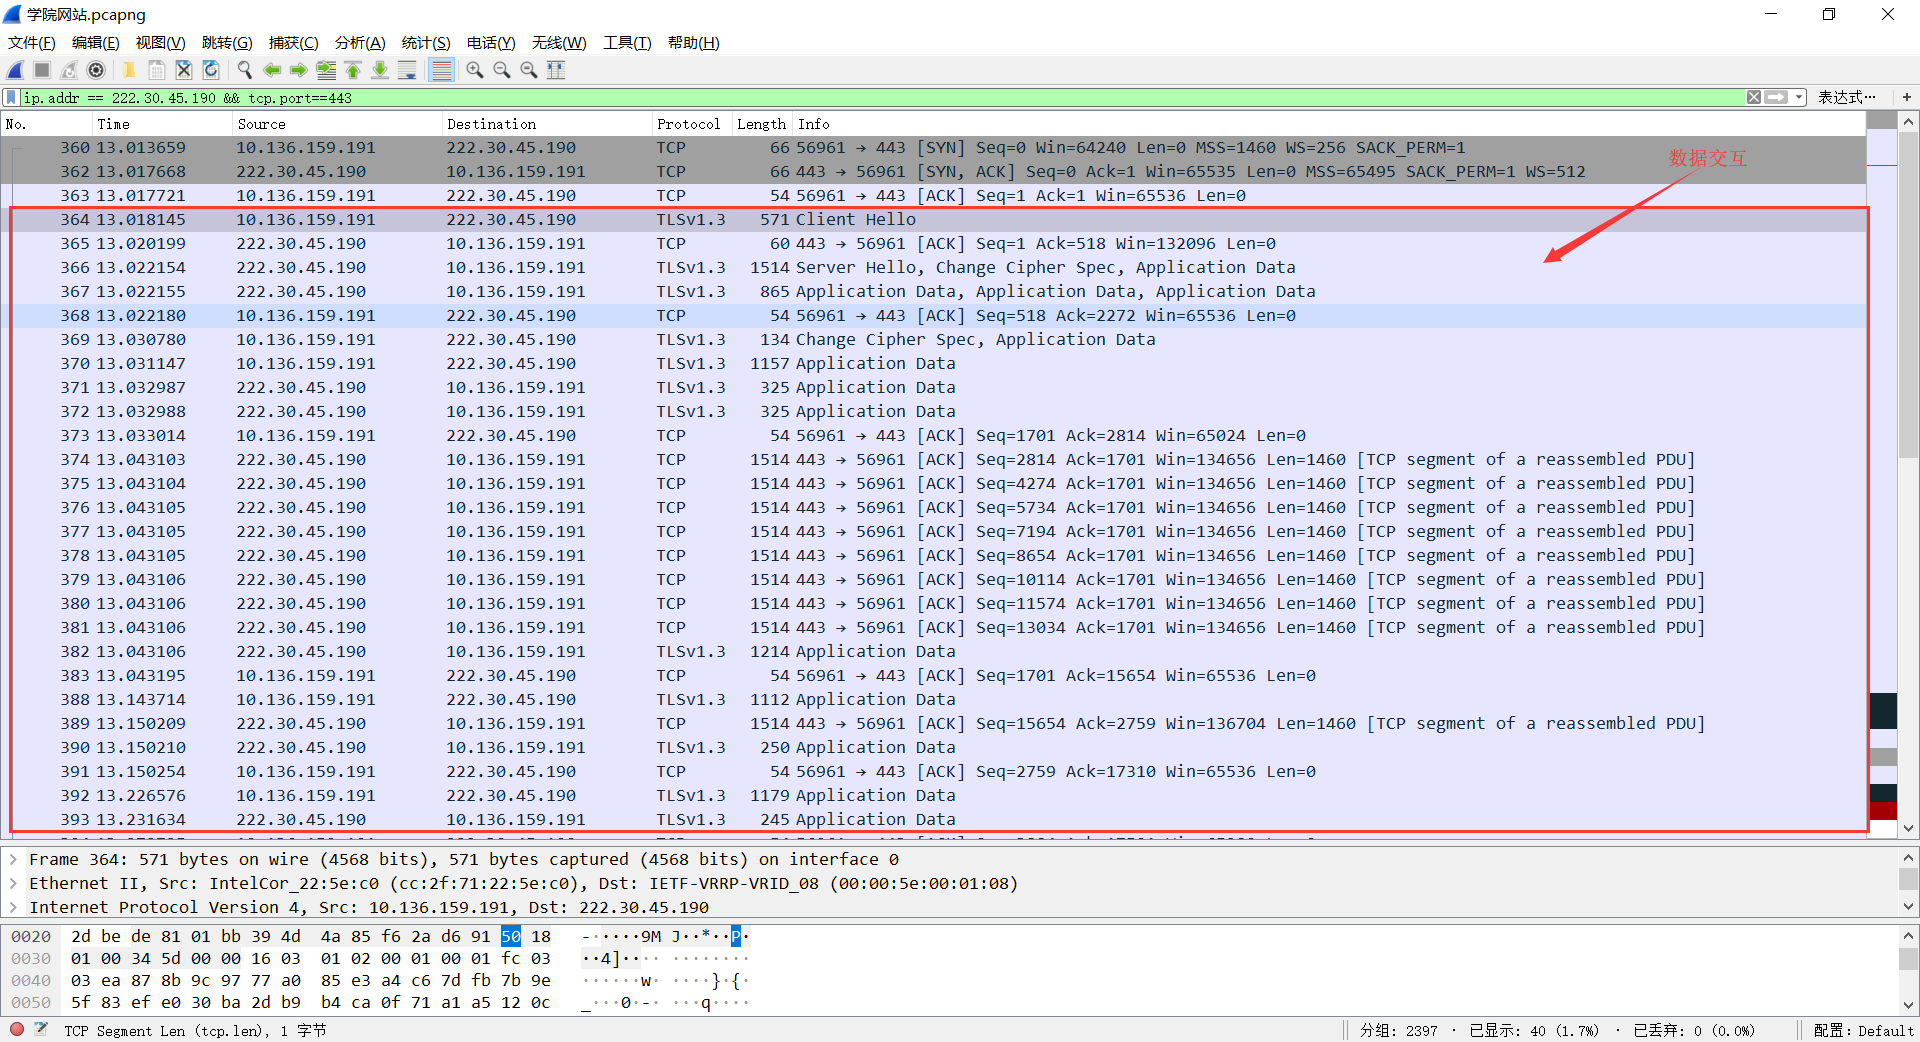
\includegraphics[width=0.65\textwidth]{数据交互}
	\caption{数据传输过程 \label{fig:10}}
\end{figure}

第一种为单个数据包的收发,即客户端发送单一的数据包,服务器端进行响应,这个过程不会涉及数据包的乱序问题,比较简单,数据收发的过程如\figref{fig:8}、\figref{fig:9}所示:
\begin{figure}[htbp]
	\centering
	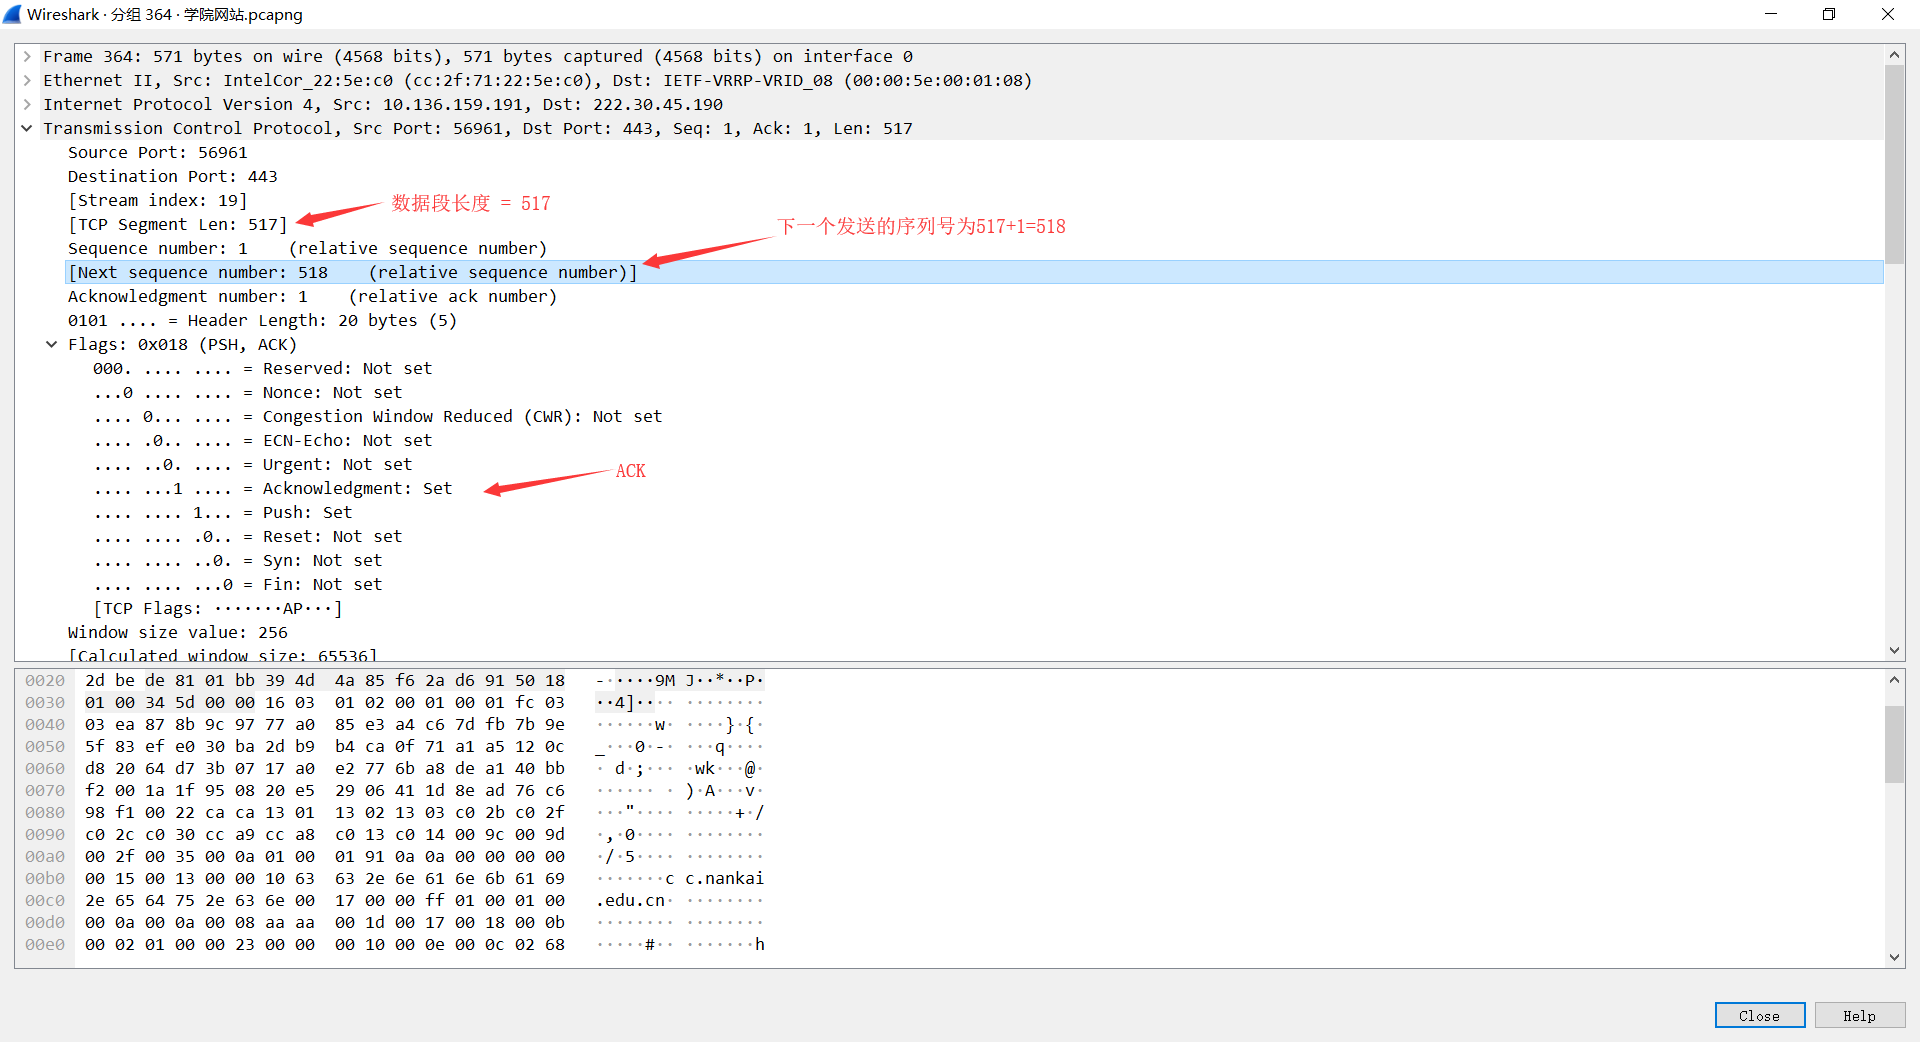
\includegraphics[width=0.8\textwidth]{data1}
	\caption{客户端发送数据包 \label{fig:8}}
	\centering
	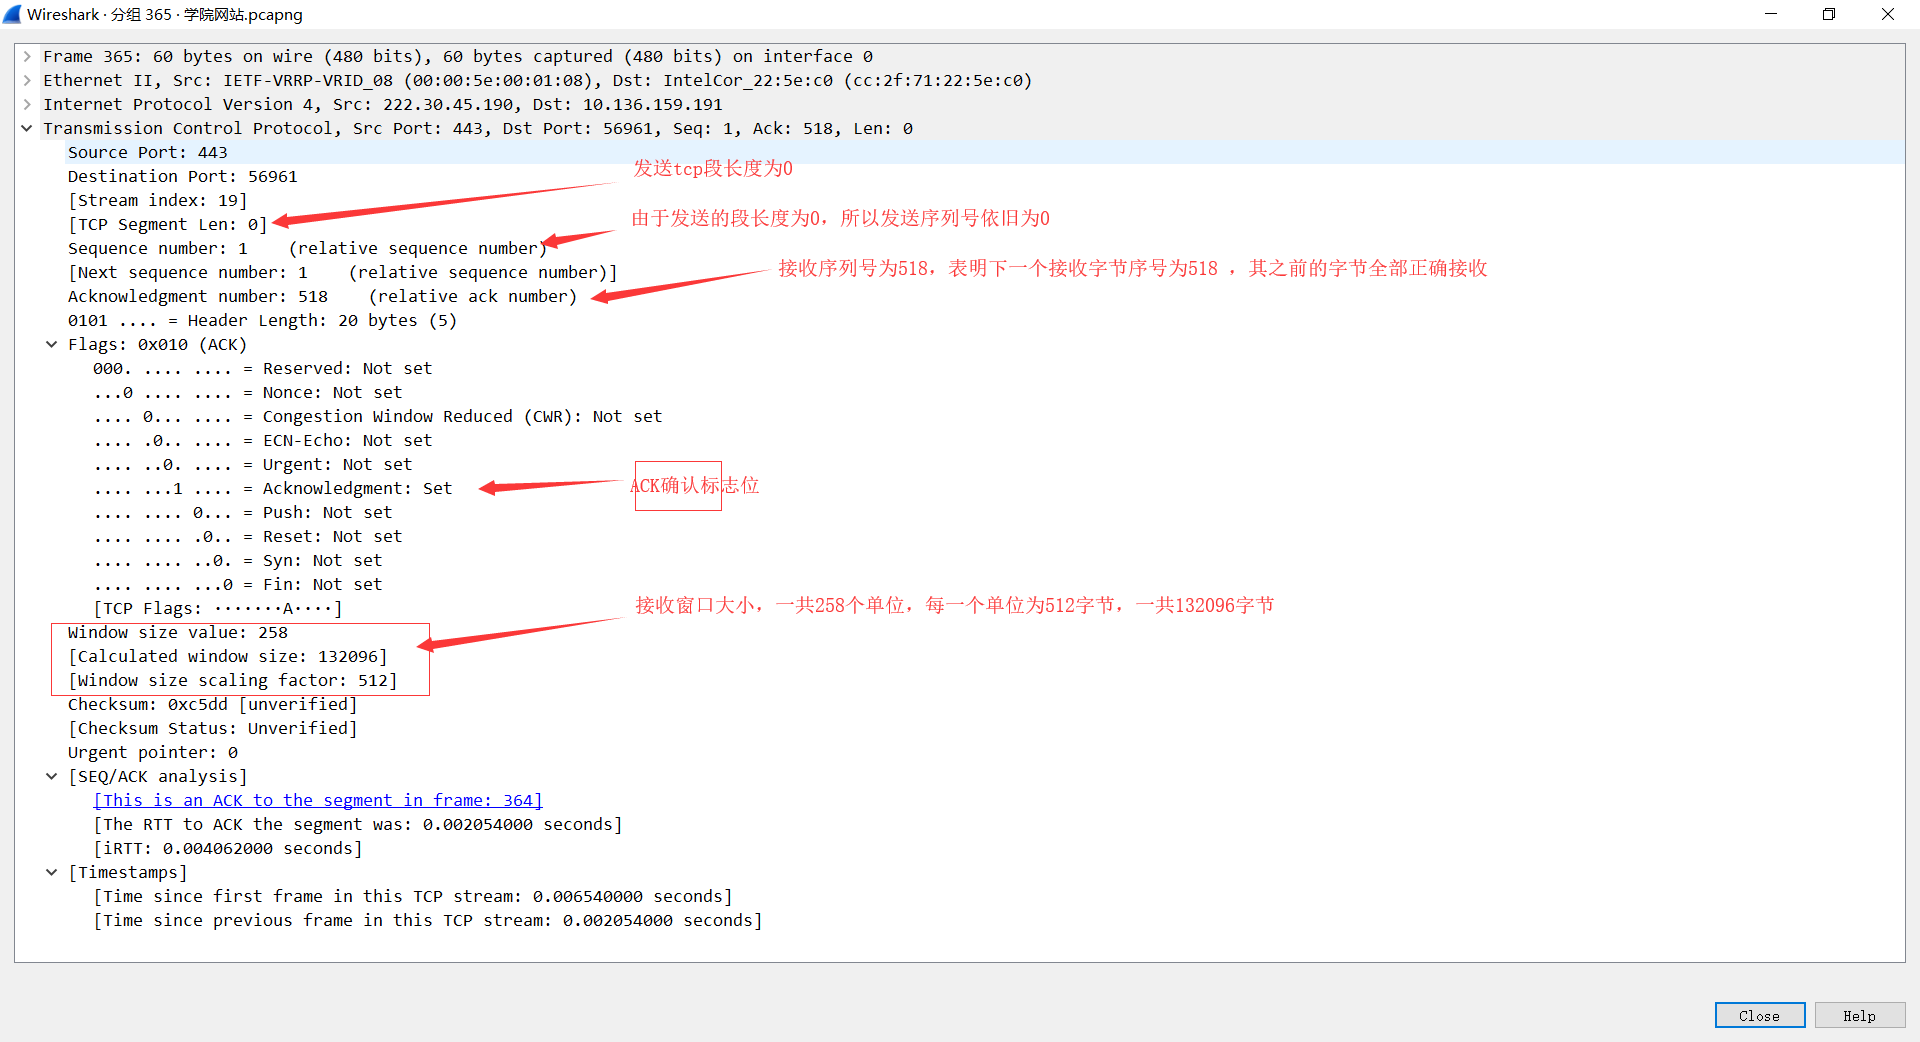
\includegraphics[width=0.8\textwidth]{data1-ACK}
	\caption{服务器确认数据包 \label{fig:9}}
\end{figure}


从\figref{fig:8}可以看到,数据段长度为517字节,发送序列号为1,同时确认了第三次握手的服务器回复数据包,在\figref{fig:9}中可以看到回复数据包的数据段长度为0,ack序号为518,为517+1,由于长度为0,所以发送序列号仍然为1。


值得说明的是,这条数据交互基于\text{TLS handshack protocol},\text{TLS}握手协议,TLS握手协议在客户和服务器进程之间协商它们在安全信道中要使用的安全参数,这些参数包括要采用的协议版本、加密算法和密钥。另外客户要认证服务器,服务器则可以选择认证或不认证客户。握手协议工作过程如下:

\begin{itemize}
	\item  客户端发送Client Hello报文给服务器端,服务器回答Server Hello。
	\item  服务器端发送Certificate报文传送数字证书和公钥。
	\item  服务器端请求客户端证书时,客户端要返回证书或返回没有证书的指示。
	\item  服务器此时要返回改变加密规范协议报文和Encrypted Handshake报文,以示完整的握手消息交换已经全部完成。
	\item  握手协议完成后,客户端即可与服务器端传输应用加密数据,应用数据加密一般是用第①步密钥协商时确定的对称加密密钥,如DES、3DE等。非对称密钥一般为RSA,用于数字证书的验证。
\end{itemize}

本次数据包即为客户端发送给服务器端的Client  Hello 报文,在此报文中设定了注入加密算法,协议版本、压缩算法之类的安全参数,截图如\figref{fig:11}所示:

\begin{figure}[htbp]
	\centering
	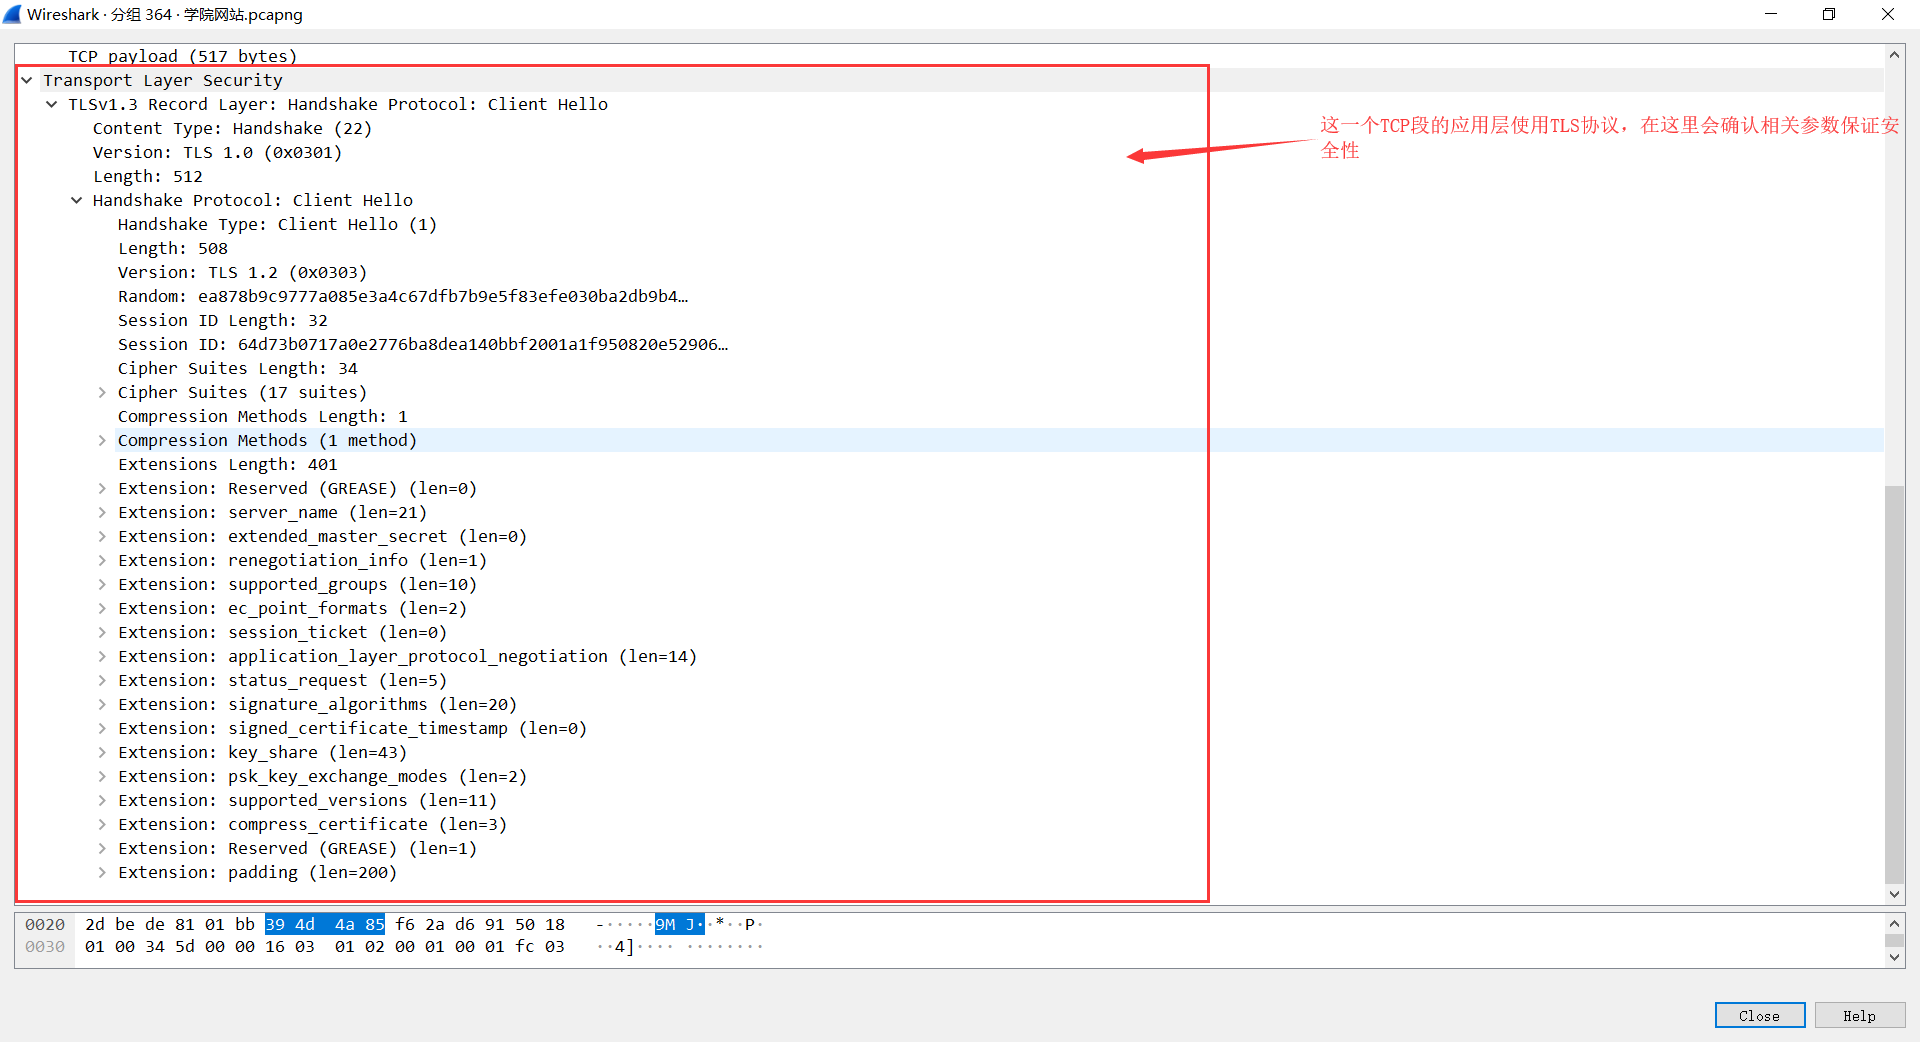
\includegraphics[width=0.6\textwidth]{data1-tls}
	\caption{TLS握手协议 \label{fig:11}}
\end{figure}

第二种数据收发即为发送端的数据包连续发送,从\figref{fig:14}中可以看到,服务器端连续向客户端发送了多条数据包,这种情况一般出现在数据包大小太大,而发送的端最大长度限制为1460字节,所以需要分多个数据包进行发送。

\begin{figure}[htbp]
	\centering
	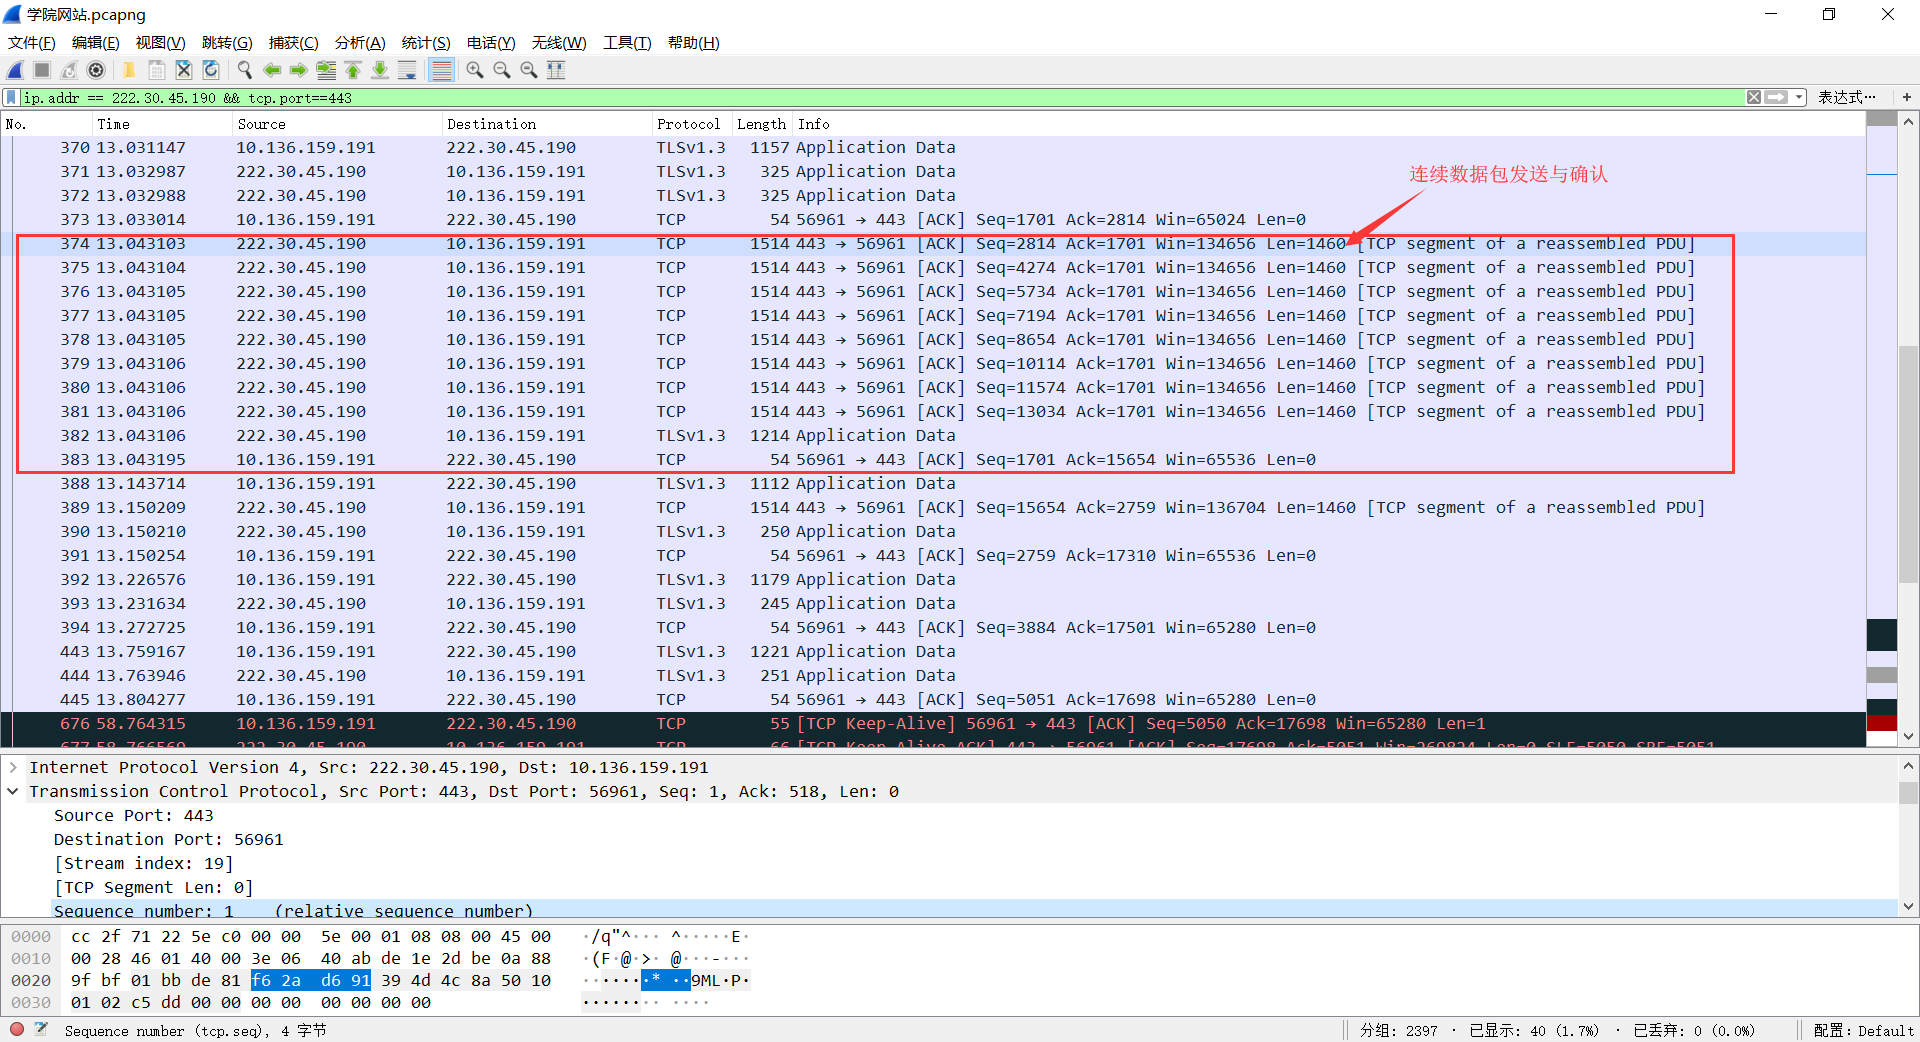
\includegraphics[width=0.8\textwidth]{连续数据包发送与确认}
	\caption{TLS握手协议 \label{fig:14}}
\end{figure}

我们可以看到在服务器端连续发送多个数据包之后,客户端只发送了一条ACK报文,这种情况体现了TCP协议中的累计确认机制,我们关注连续发送的最后一条报文如\figref{fig:12}:

\begin{figure}[htbp]
	\centering
	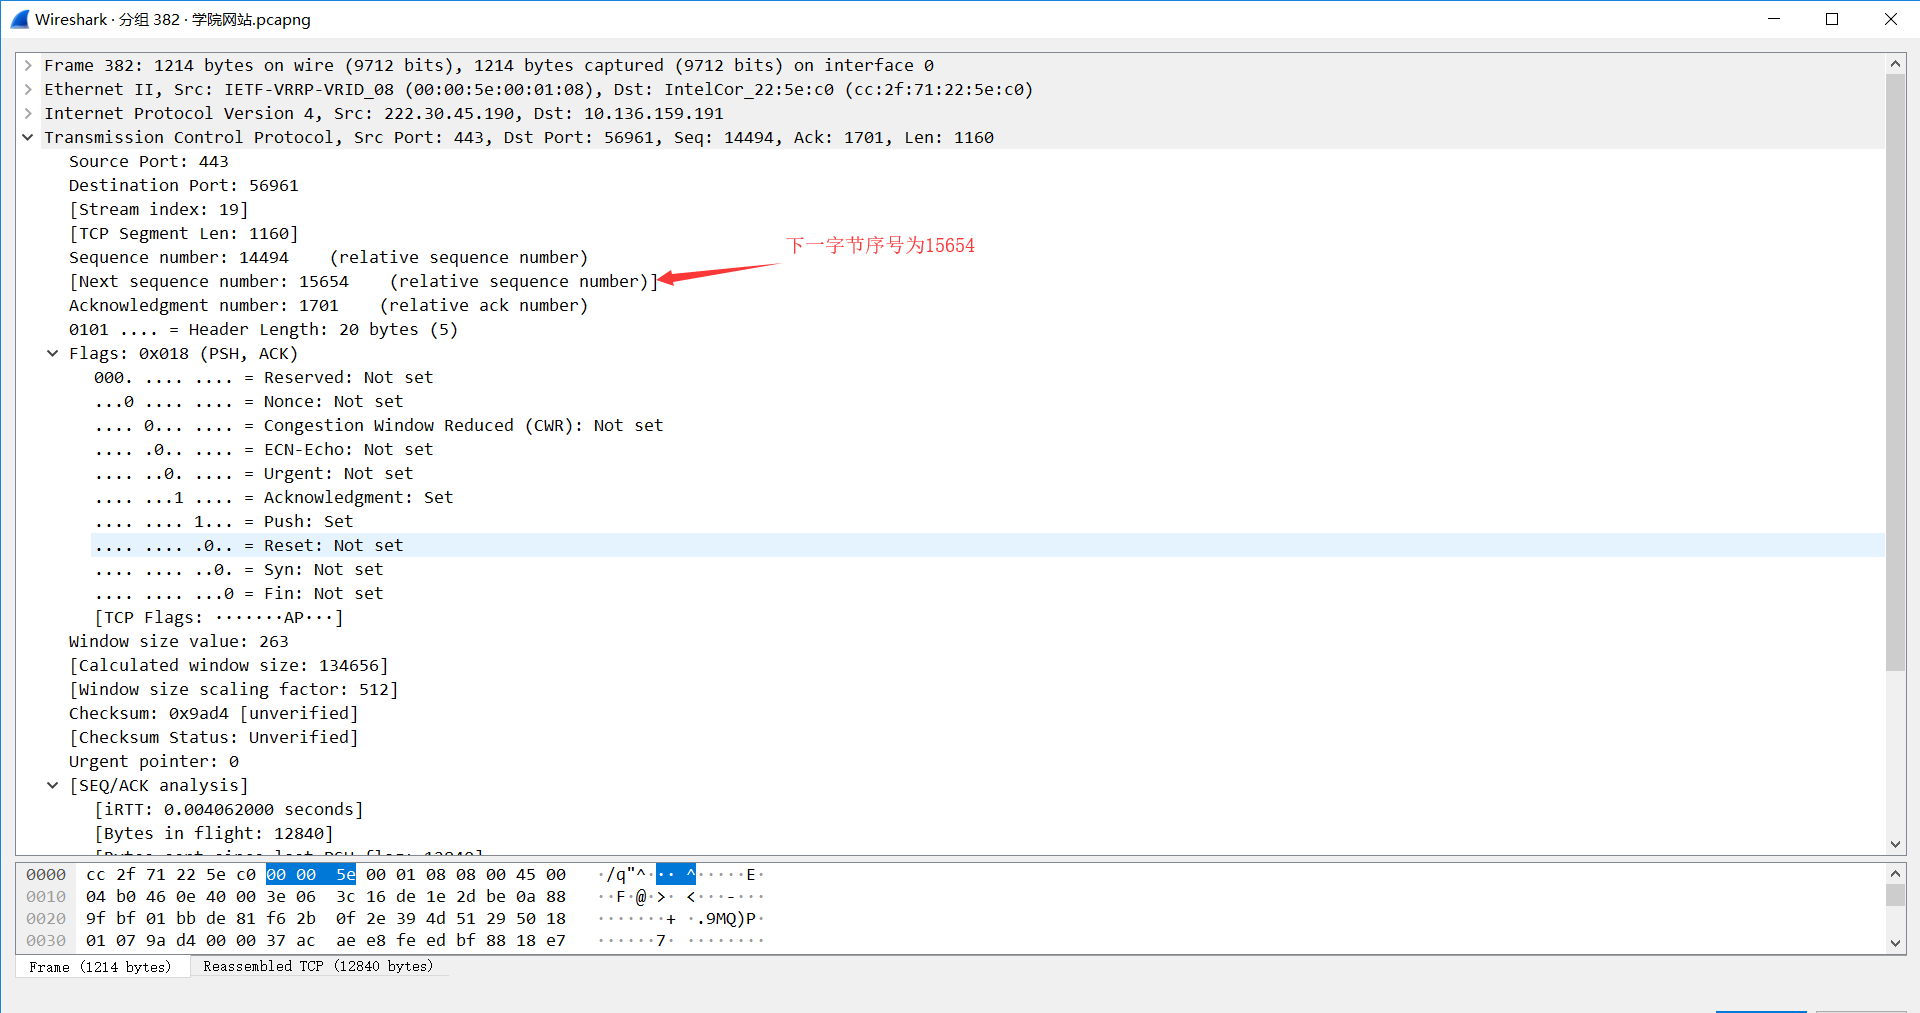
\includegraphics[width=0.8\textwidth]{连续数据包发送nextseq}
	\caption{服务器连续发送最后一个数据包 \label{fig:12}}
\end{figure}

可以看到,客户只是在按序接受了所有连续发送的数据包之后才回复了一条ACK报文。

\subsubsection{PUSH字段作用}

通常来说当接收放接收数据之后,在什么时间将缓冲区哪些数据包发往上层应用是由接收方自行决定的,但是当出现上述的将大文件拆分成多个文件的情况下,让接收方自行决定推送方式可能会导致接收方应用层一次接受的数据不完整,因此对发送方来说,会将分拆打包成TCP报文的多个数据包的最后一个TCP报文flags中的PUSH字段置为1,要求接收方在接收发到包含PUSH字段的TCP报文时,立即将缓冲区中已经接收到的报文传给上层应用。

除此之外,如果应用层希望自己的数据能够立即发送出去而不是在发送缓冲区中等待,可以添加PUSH字段,这样发送端会优先发发送带有PUSH字段的报文,当然如果缓冲区满了,TCP同样会将发送缓冲区中的所有数据打包发送。

在上述分析中的\figref{fig:12}中可以看到PUSH字段被置位为1,原因即是因为该报文为打包发送的最后一个报文,为了快速发送以及在接收方能够尽快传给上层应用,使用了PUSH标志位。
\subsubsection{TCP Keep-alive机制}

在本次的实验中出现了TCP keep-alive机制,这种机制出现在,当服务器客户端经过一定时间未通信之后,客户端会发送一条带有一个字节0数据的keep-alive报文区确认与服务器之间的连接是否还存在,具体报文可以看\figref{fig:13}:

\begin{figure}[htbp]
	\centering
	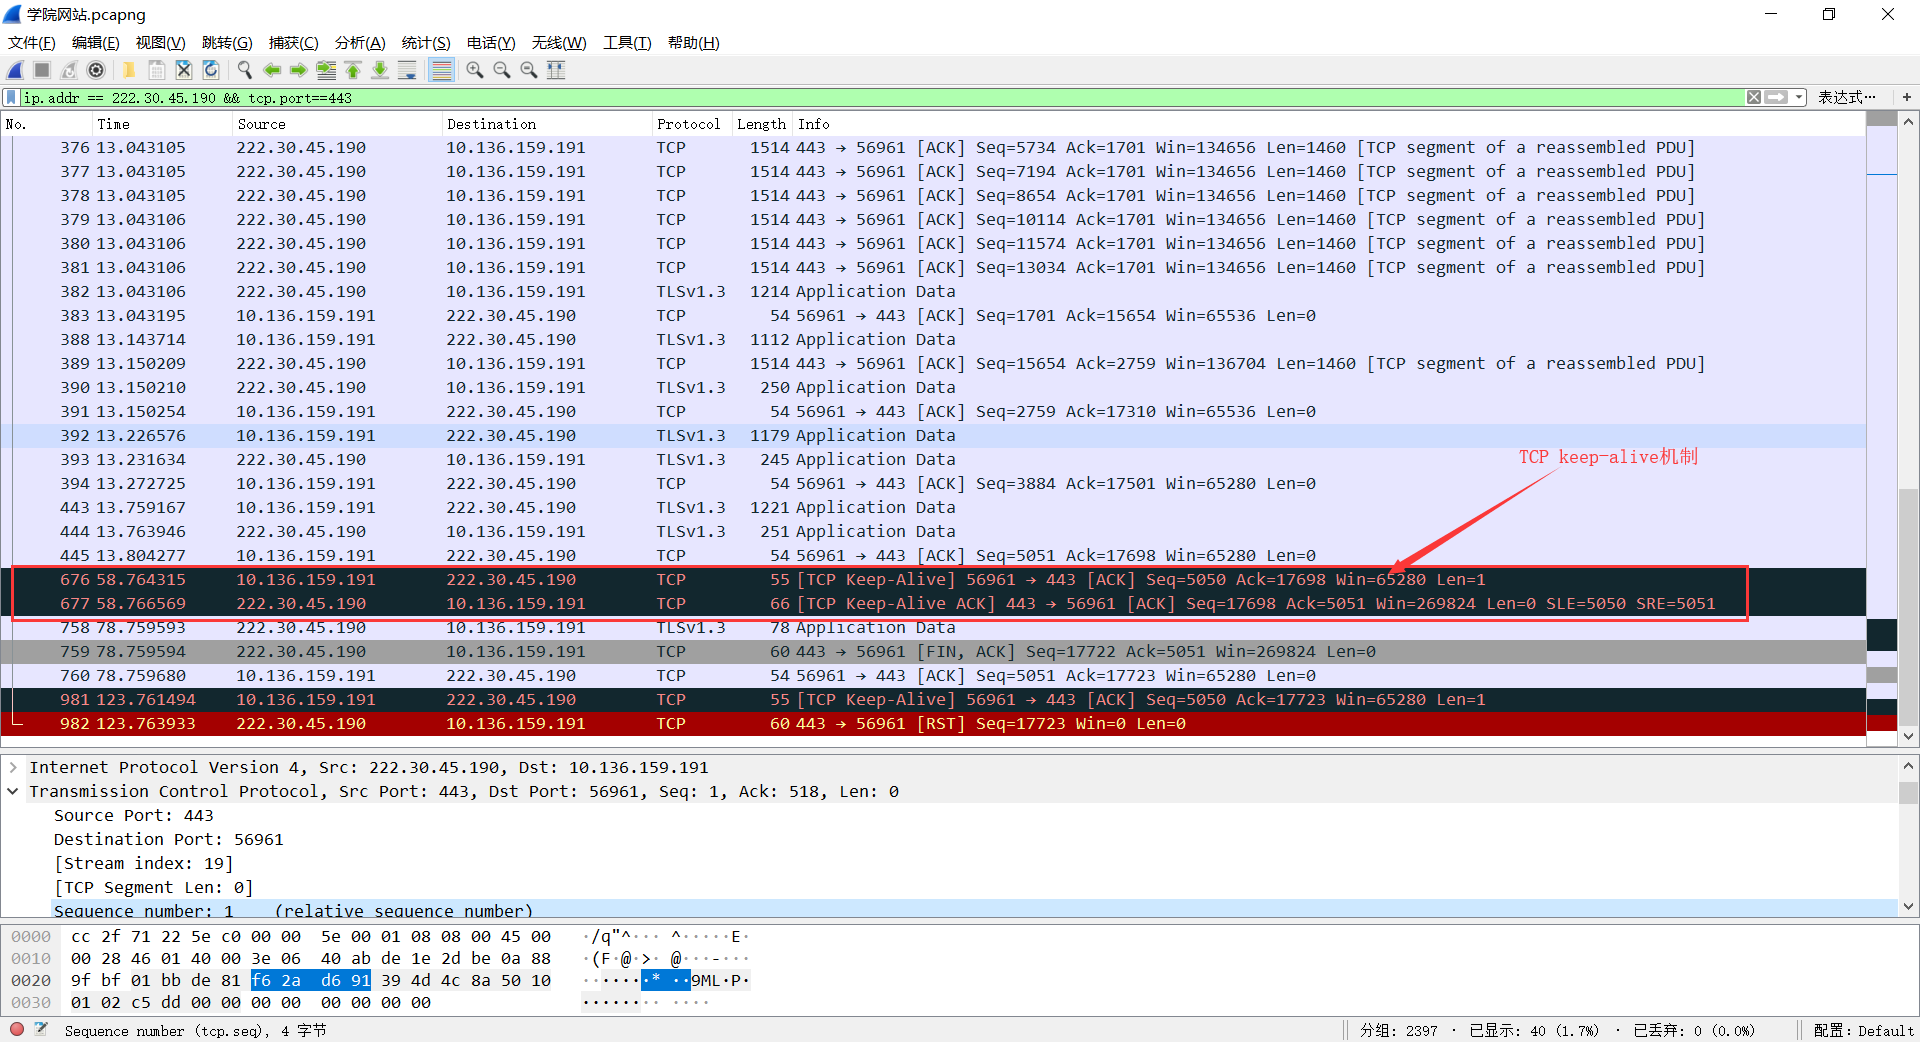
\includegraphics[width=0.8\textwidth]{tcp-keepalive}
	\caption{keep-alive报文 \label{fig:13}}
\end{figure}

服务器端会通过选择确认机制确认收到的这一个字节的数据,截图如\figref{fig:15}所示:

\begin{figure}[htbp]
	\centering
	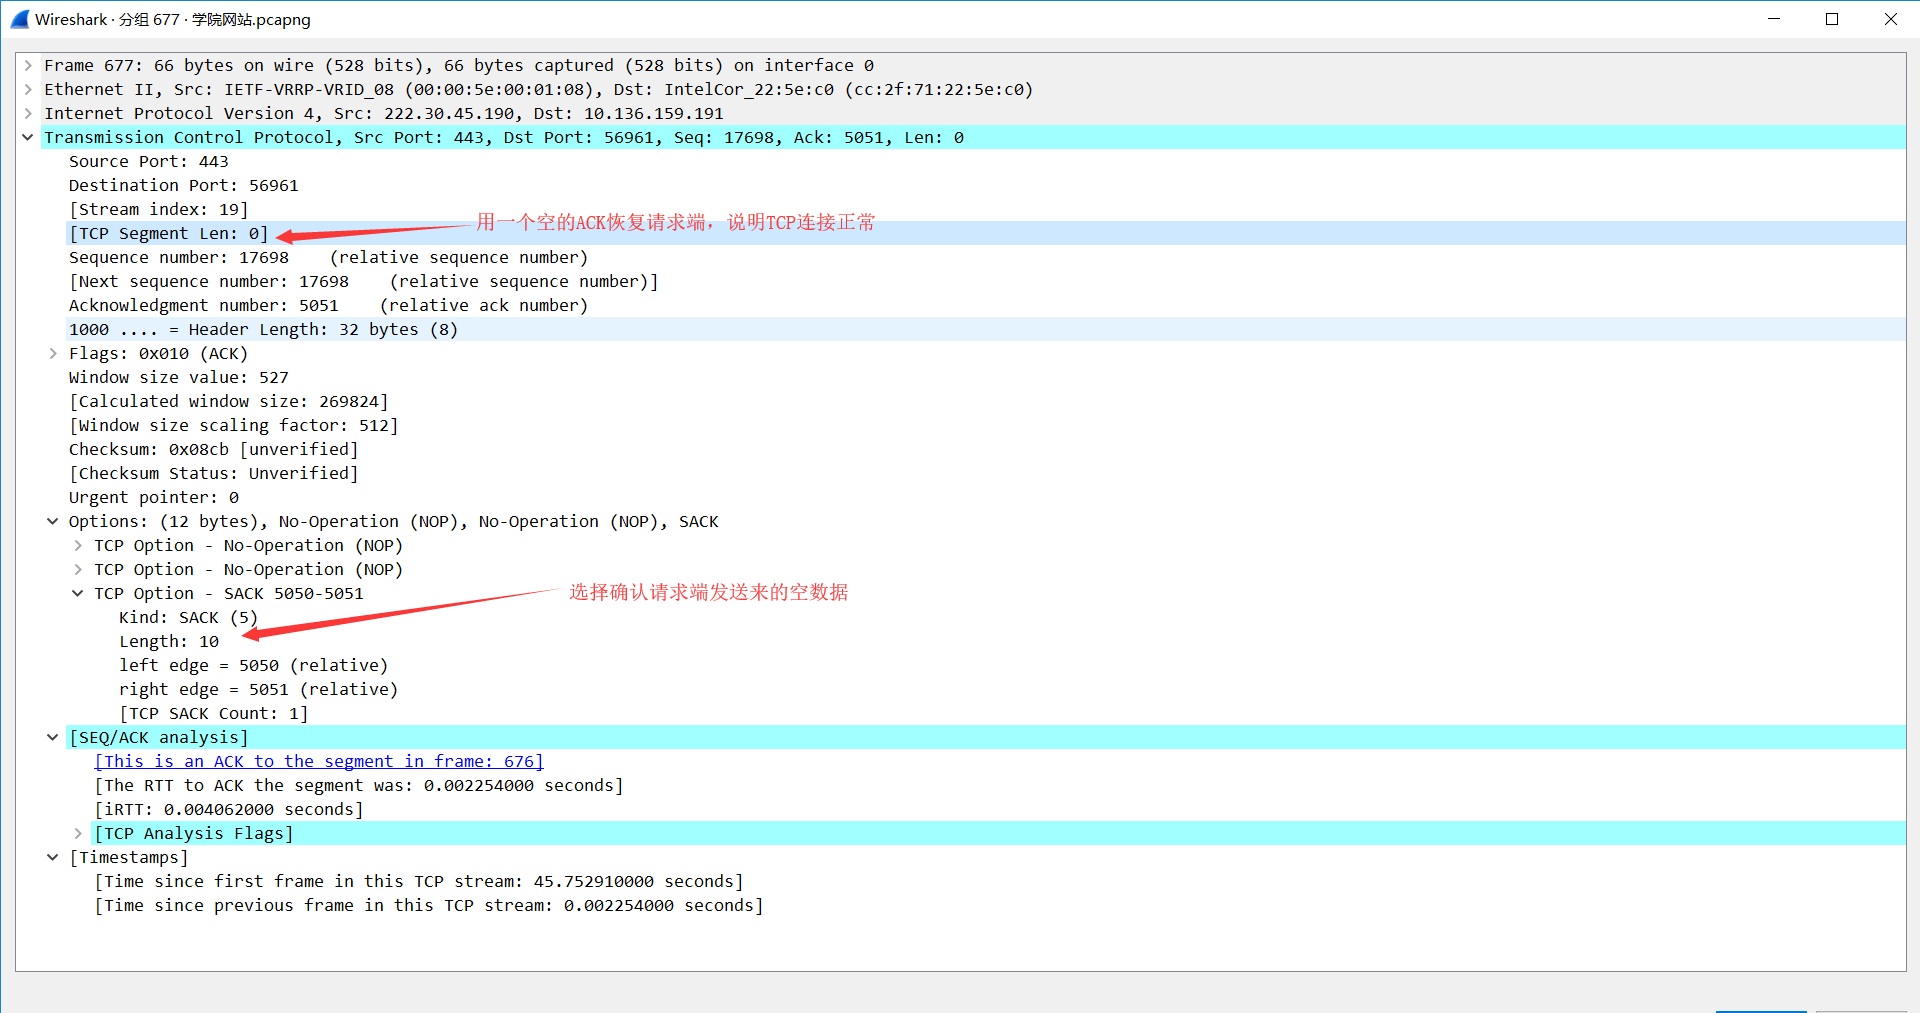
\includegraphics[width=0.8\textwidth]{keepacliveack}
	\caption{选择确认机制 \label{fig:15}}
\end{figure}

\newpage
\subsection{四次挥手拆除连接}
数据收发结束之后或者长时间连接未用,则会发起连接关闭请求,关闭连接一共分为四个过程,称为四次挥手拆除连接。拆除的过程示意图如\figref{fig:16}所示:

\begin{figure}[htbp]
	\centering
	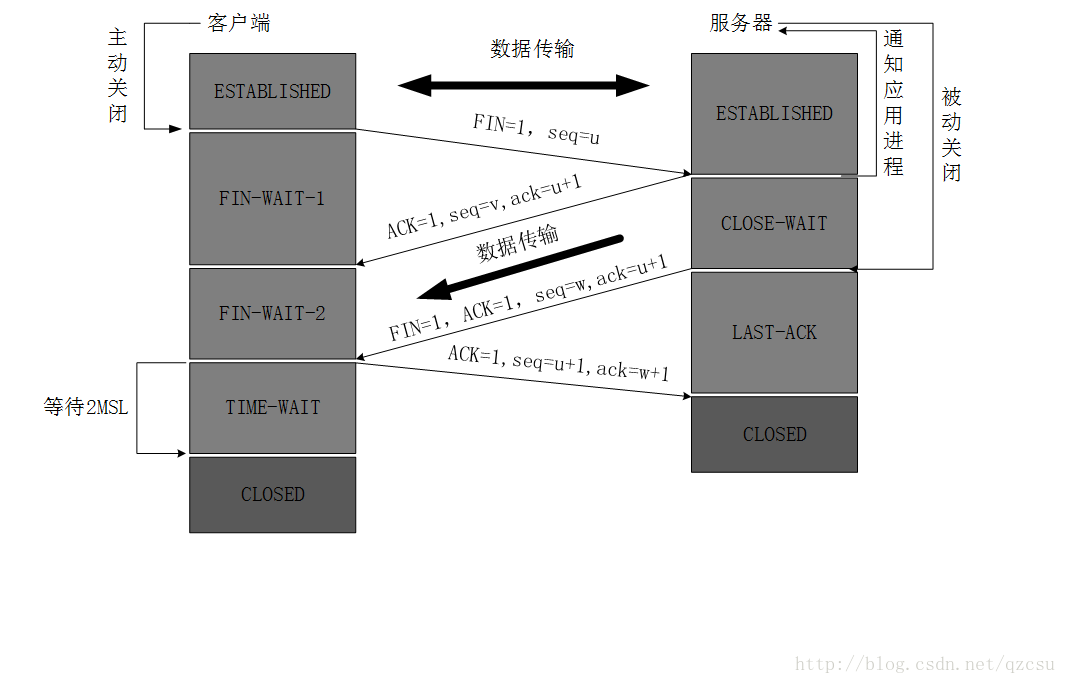
\includegraphics[width=0.8\textwidth]{四次挥手}
	\caption{四次挥手拆除连接示意图 \label{fig:16}}
\end{figure}

四次挥手所分析的数据TCP连接为TCP连接2,截图如\figref{fig:17}:

\begin{figure}[htbp]
	\centering
	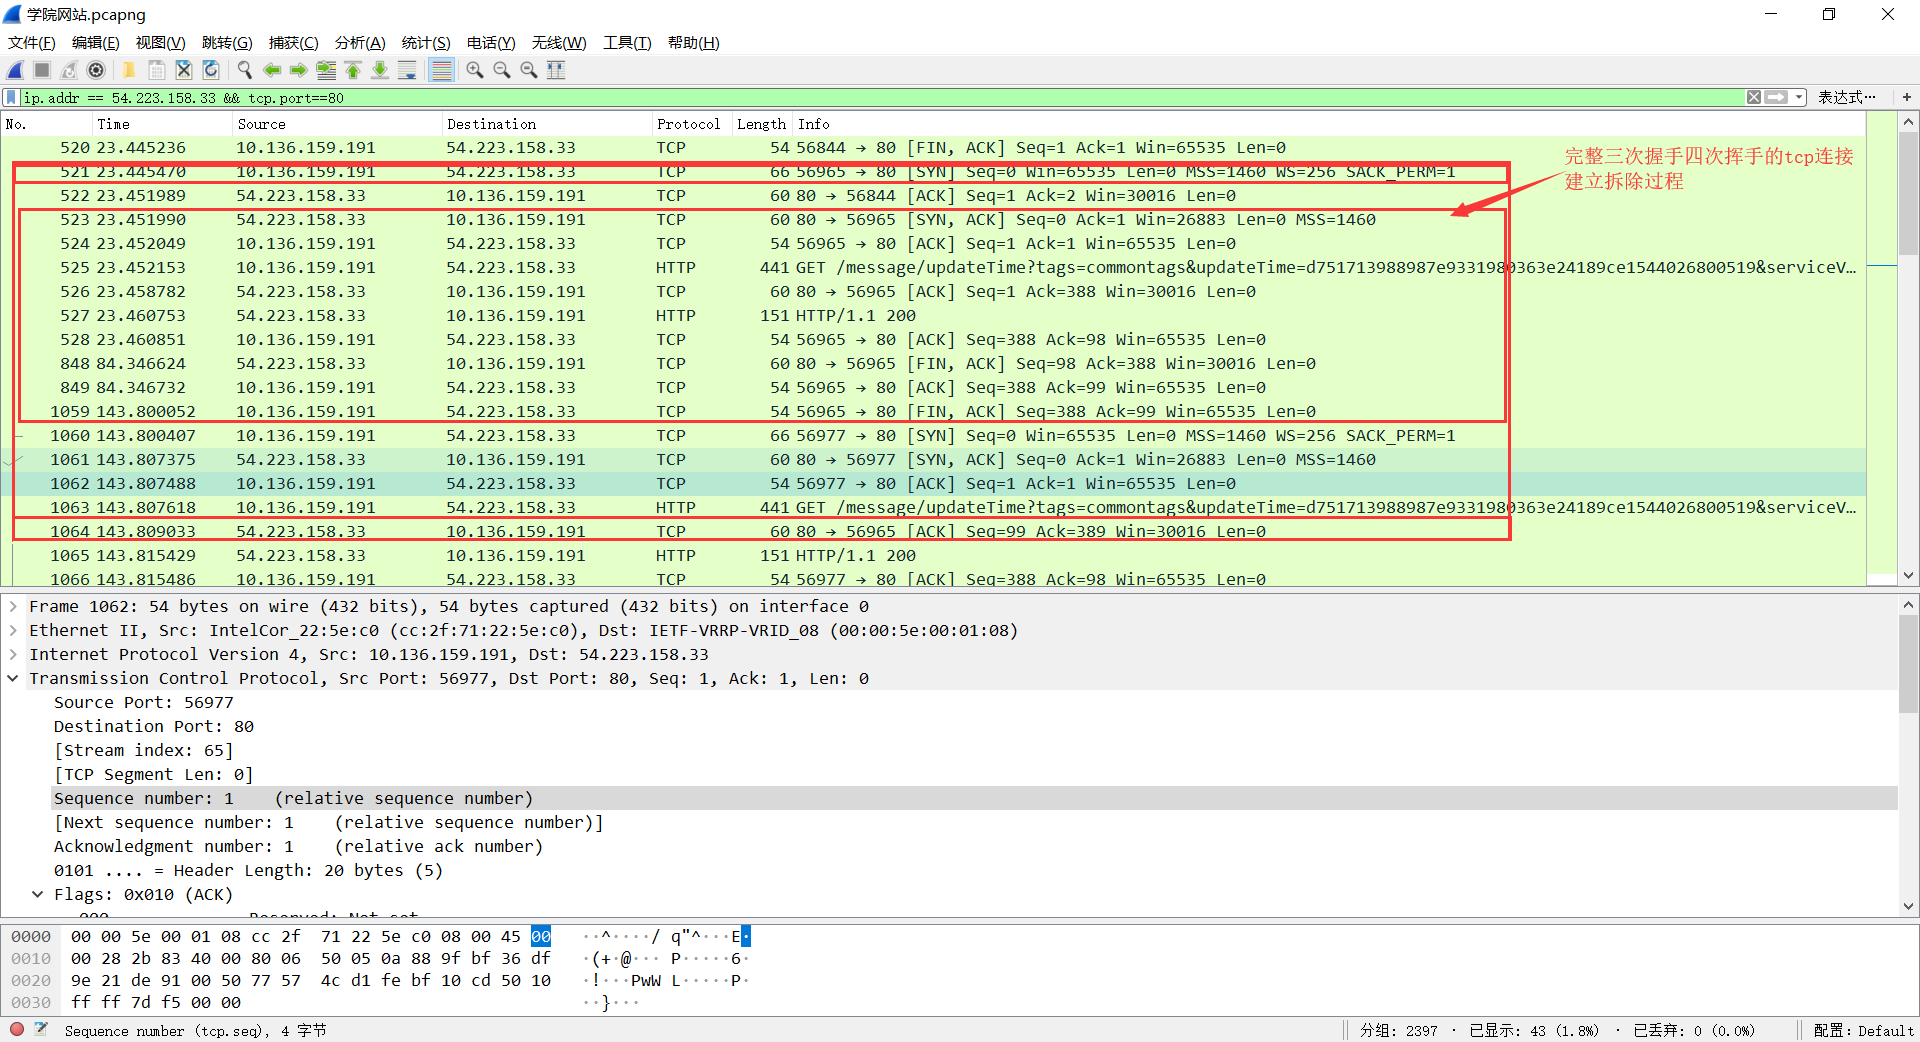
\includegraphics[width=0.8\textwidth]{完整34}
	\caption{TCP 连接2 完整的建立拆除连接截图 \label{fig:17}}
\end{figure}


\subsubsection{第一次挥手}

第一次挥手为服务器端发现没有数据收发结束之后,为节省系统资源,会发起关闭连接的请求,报文的特征为FIN位置位为1,发送完这条报文之后,服务器将不能继续发送数据报文,但是能够接收和发送ACK报文。从\figref{fig:17}可以看到该报文发送序列号为98,确认序列号为388。

\subsubsection{第二次挥手}

第二次挥手是客户端接收到服务器端发送的关闭连接请求,客户端回送一个ACK报文,说明接收到关闭请求,进入被动关闭等待状态,在此期间客户端仍然可以向服务器发送数据,这一点在TCP连接2的关闭连接过程中可以看出来。从\figref{fig:17}可以看到该报文发送序列号为388,确认序列号为99。

\subsubsection{第三次挥手}


第三次挥手为客户端继续发送一条FIN段,说明自己进入关闭等待状态,等待服务器端回送ACK进行关闭,在此期间客户端无法继续发送数据。从\figref{fig:17}可以看到该报文发送序列号为388,确认序列号为99,之所以序列号没有改变是由于这两条报文并没有携带数据段。


\subsubsection{第四次挥手}

当服务器接收到客户端的ACK报文之后,进入到关闭等待状态2,等待接收客户端的FIN段。接收到客户端的FIN字段报文之后,回送一个ACK回复,从\figref{fig:17}可以看到该报文发送序列号为99,确认序列号为389。开始计时后经过2倍的TCP生存周期之后关闭TCP连接,同时在客户端接收到ACK回复之后立即关闭连接。

\subsubsection{reset快速拆除连接}

在TCP连接1中,经过两次挥手之后,在服务器端接收到来自客户端对于关闭连接请求的ACK报文之后,直接发送了一条RESET命令快速拆除与客户端之间的连接,利用RST位进行复位的时候,不必等待缓冲区中的包都发出,而是可以直接发送RST段后关闭连接,而客户端接收到RST段后也不必回复ACK,可直接关闭连接。一般来说RST段用来关闭异常连接,但是也有的情况会被用来快速关闭连接,减少关闭连接时的交互。

拆除TCP连接1的过程即数据包的结构截图如下所示:

\begin{figure}[htbp]
	\centering
	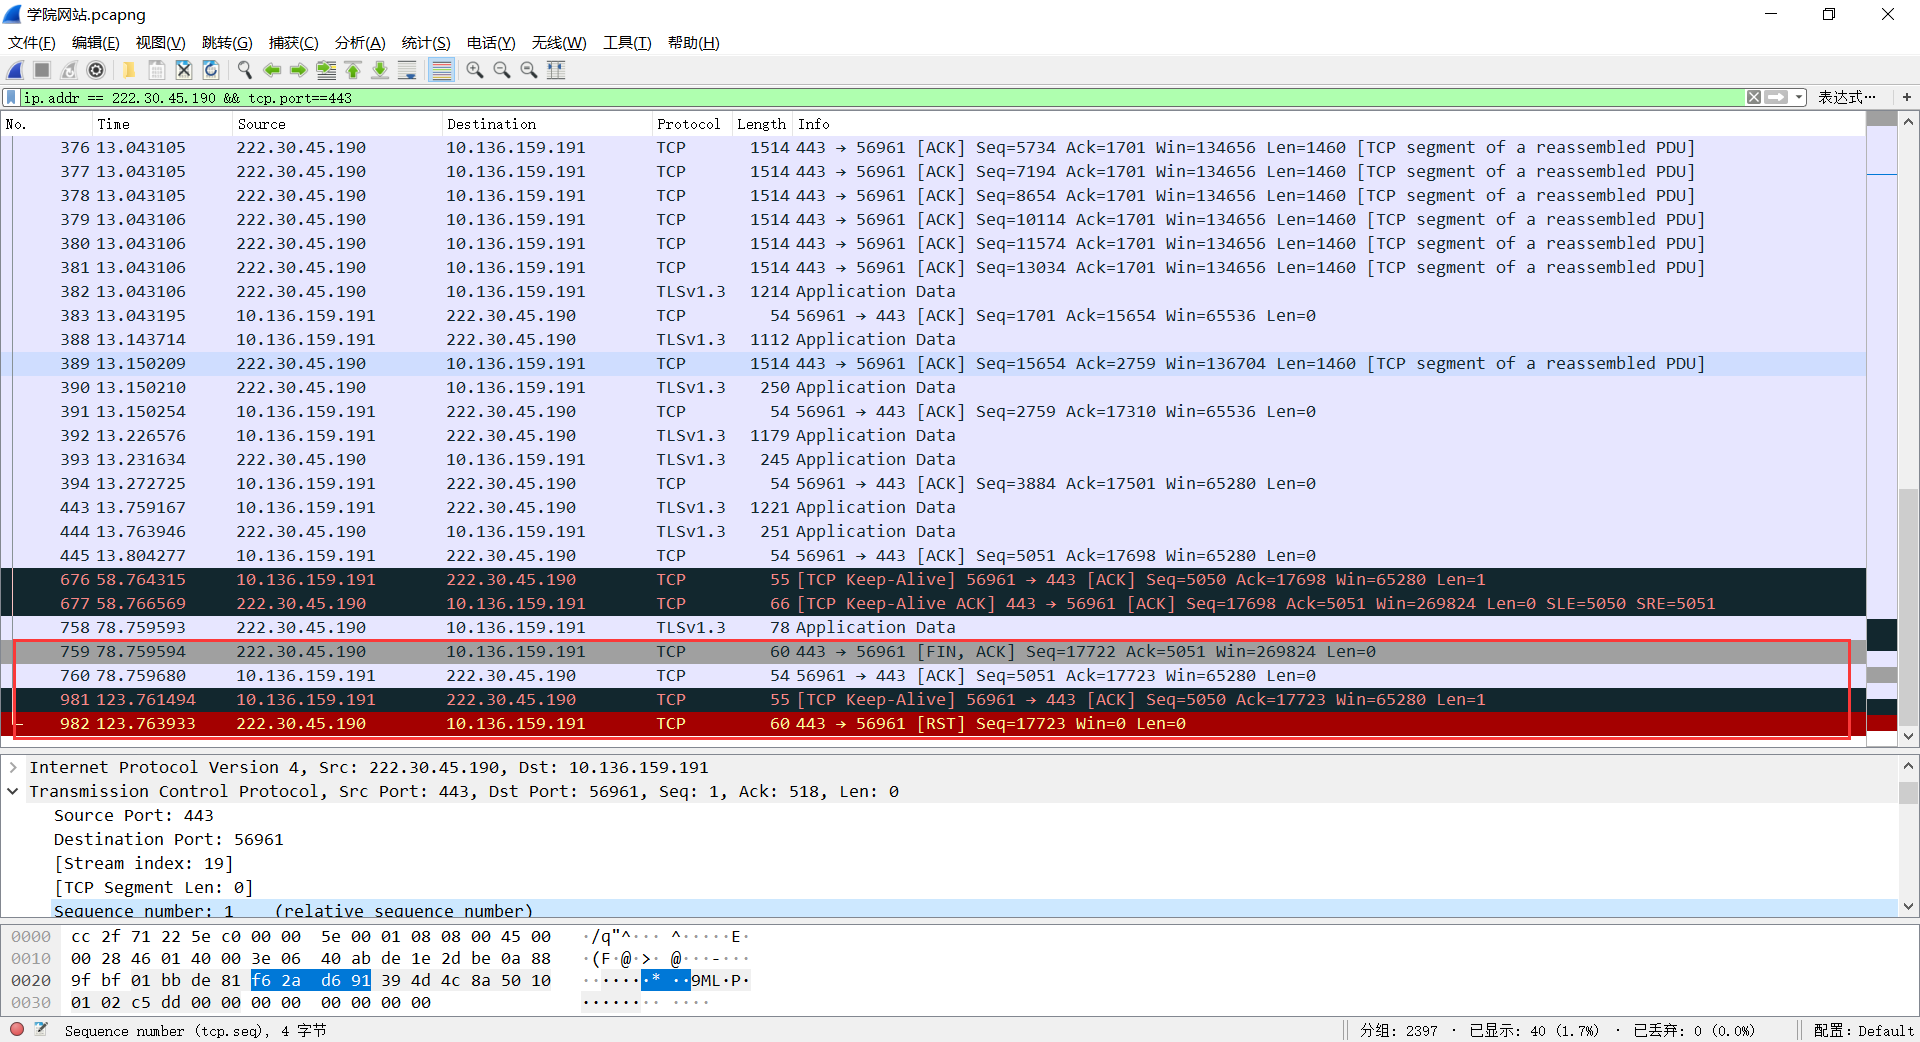
\includegraphics[width=0.8\textwidth]{连接拆除}
	\caption{TCP 连接1 拆除连接截图 \label{fig:18}}
	\centering
	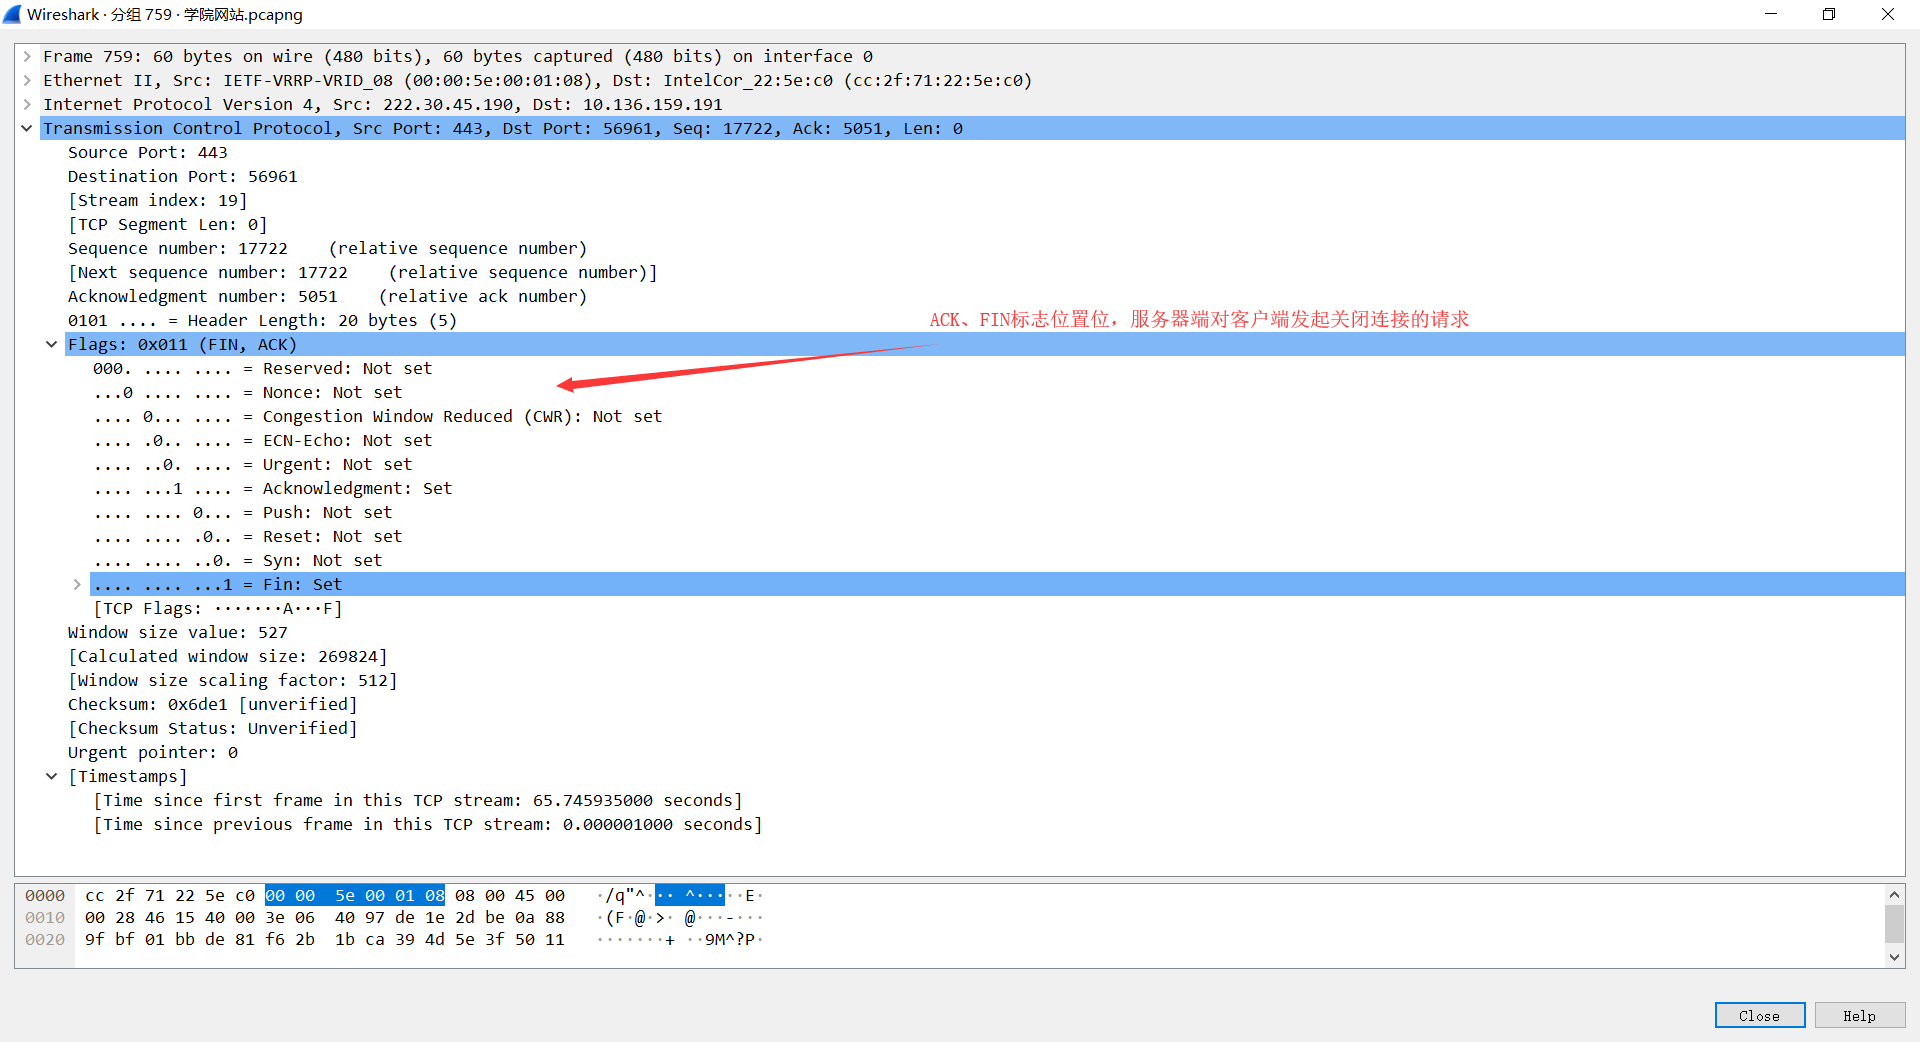
\includegraphics[width=0.8\textwidth]{关闭连接-server}
	\caption{TCP 连接1 服务器发出关闭连接报文结构 \label{fig:19}}
	\centering
	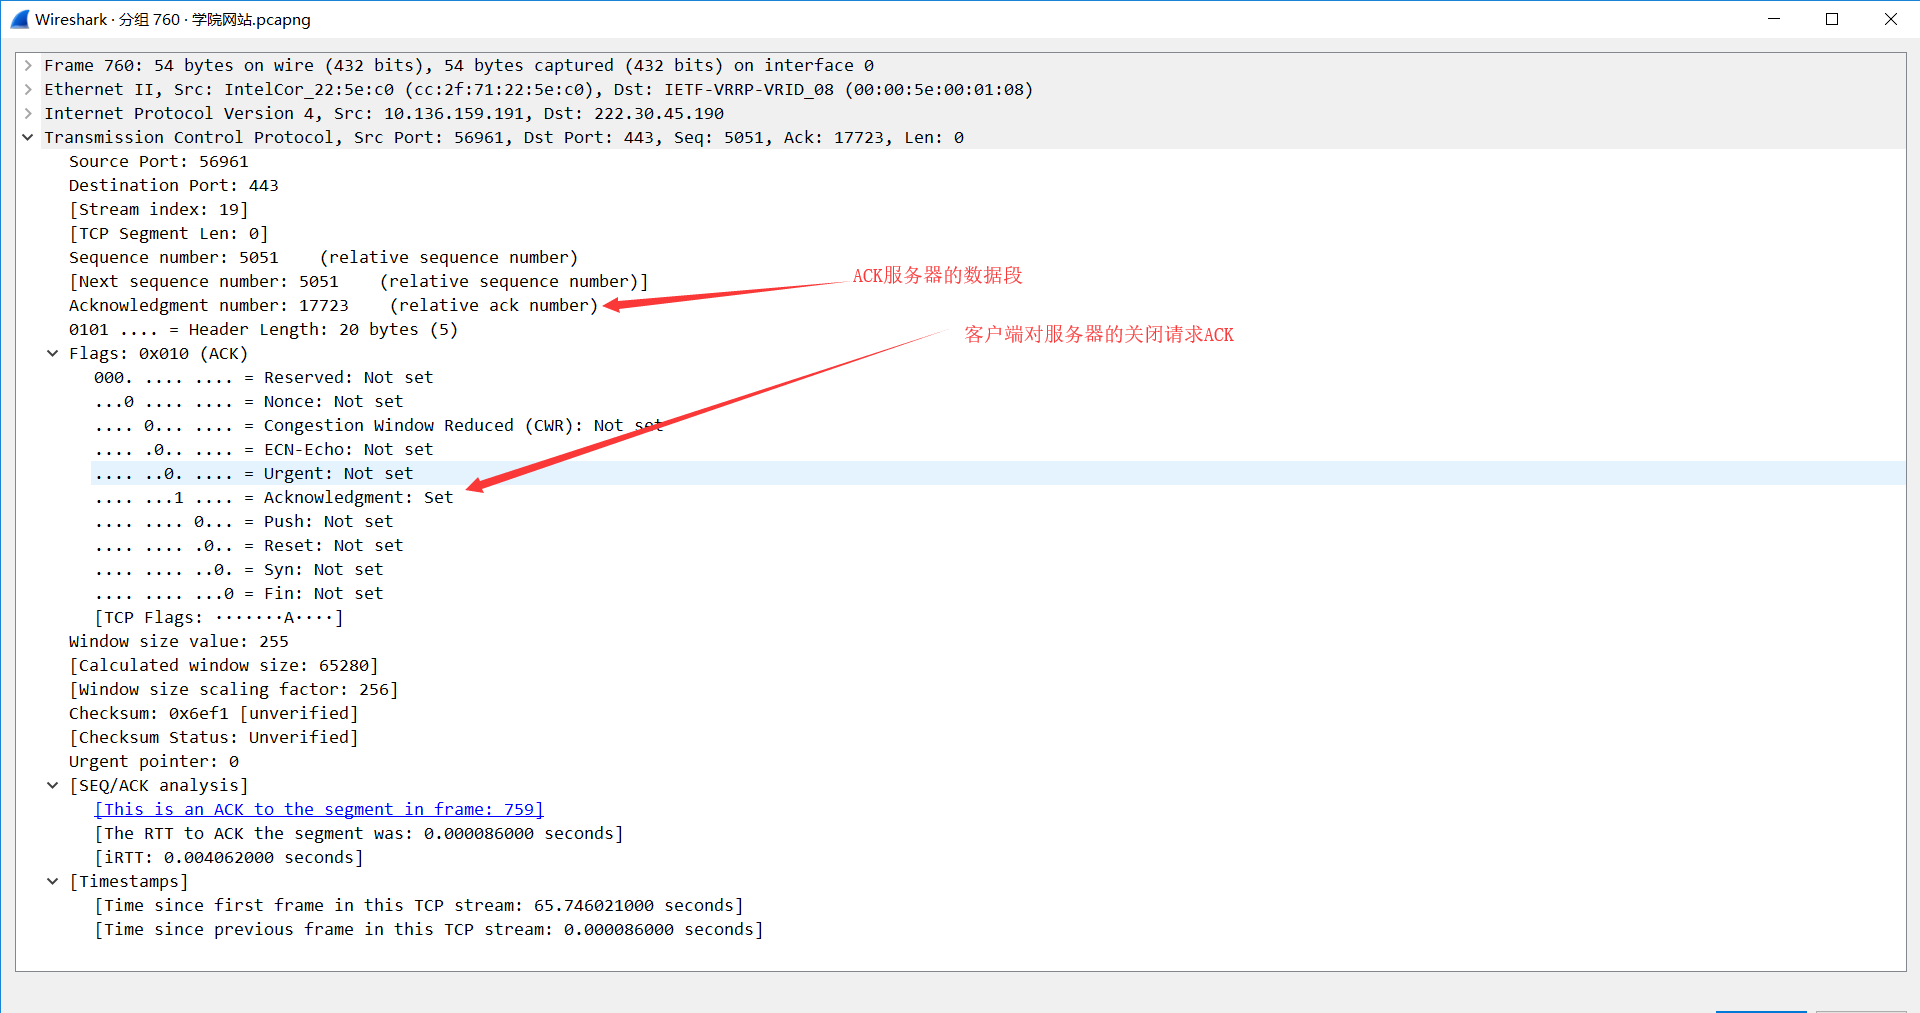
\includegraphics[width=0.8\textwidth]{关闭连接ack}
	\caption{TCP 连接1 客户端回复ACK报文结构\label{fig:20}}
\end{figure}

\newpage
\section{总结与思考}
在本次TCP数据包分析中发现了在实际情况下,TCP连接的建立和拆除以及数据传输过程和课堂上所学的还是存在一定的区别,比如在拆除连接的过程中,一般情况下课堂上所介绍的都是四次挥手过程拆除TCP连接,但是在这次分析的实际数据保重可以看出,也存在一些情况下使用RST段来快速关闭连接,此外在实际的数据传输过程中也有使用push字段来强制将报文立即发送的情况,以及使用keep-alive机制来保证连接的稳定性。

总而言之,通过这次对于TCP数据包的分析和TCP连接的建立拆除分析,我对于在课堂上所了解的TCP协议有了更深刻的认识,也对于WireShark这个工具使用的更加熟练了。

\section{参考资料}
[1] 维基百科.传输控制协议.https://zh.wikipedia.org/wiki/\%E4\%BC\%A0\%E8\%BE\%93\%E6\%8E\%A7
    \%E5\%88\%B6\%E5\%8D\%8F\%E8\%AE\%AE

[2] 百度百科.握手协议.https://baike.baidu.com/item/\%E6\%8F\%A1\%E6\%89\%8B\%E5\%8D\%8F\%E8
    \%AE\%AE/4058729?fr=aladdin

\nocite{*}

% 如果想修改参考文献样式(非国标),请把下行取消注释,并换成合适的样式(比如 unsrt,plain 样式)。
%\bibliographystyle{aer}
%\bibliography{wpref}

\end{document}
